%%%%%%%%%%%%%%%%%%%%%%%%%%%%%%%%%%%%%%%%%%%%%%%%%%%%%%%%%%%%%%%%%%%%%
% LaTeX Template: Project Titlepage Modified (v 0.1) by rcx
%
% Original Source: http://www.howtotex.com
% Date: February 2014
% 
% This is a title page template which be used for articles & reports.
% 
% This is the modified version of the original Latex template from
% aforementioned website.
% 
%%%%%%%%%%%%%%%%%%%%%%%%%%%%%%%%%%%%%%%%%%%%%%%%%%%%%%%%%%%%%%%%%%%%%%

\documentclass[12pt]{article}
\usepackage[a4paper]{geometry}
\usepackage[myheadings]{fullpage}
\usepackage{fancyhdr}
\usepackage{lastpage}
\usepackage{wrapfig, subcaption, setspace, booktabs}
\usepackage[final]{graphicx}
\usepackage[T1]{fontenc}
\usepackage[font=small, labelfont=bf]{caption}
\usepackage{subcaption}
\usepackage{fourier}
\usepackage[protrusion=true, expansion=true]{microtype}
\usepackage[english]{babel}
\usepackage{sectsty}
\usepackage{url, lipsum}
\usepackage{tgbonum}
\usepackage{hyperref}
\usepackage{xcolor}
\usepackage{placeins}
\usepackage{cleveref}
\usepackage{multicol}

\newcommand{\HRule}[1]{\rule{\linewidth}{#1}}
\onehalfspacing
\setcounter{tocdepth}{5}
\setcounter{secnumdepth}{5}

\newcommand{\AuAu}{Au$+$Au}
\newcommand{\PbPb}{Pb$+$Pb}
\newcommand{\sNN}{$\sqrt{s_{NN}}$}
\newcommand{\RHIC}{RHIC}
\newcommand{\STAR}{STAR}
\newcommand{\ALICE}{ALICE}
\newcommand{\TPC}{TPC}
\newcommand{\TOF}{TOF}
\newcommand{\BBC}{BBC}
\newcommand{\DCA}{DCA}
\newcommand{\PID}{PID}

%-------------------------------------------------------------------------------
% HEADER & FOOTER
%-------------------------------------------------------------------------------
\pagestyle{fancy}
%\fancyhf{}
\setlength\headheight{15pt}
%\fancyhead[L]{Student ID: 1034511}
%\fancyhead[R]{Anglia Ruskin University}
%\fancyfoot[R]{Page \thepage\ of \pageref{LastPage}}
%-------------------------------------------------------------------------------
% TITLE PAGE
%-------------------------------------------------------------------------------

\begin{document}
{\fontfamily{cmr}\selectfont
\title{ \normalsize \textsc{}
		%\\ [1.0cm]
		\HRule{2pt} \\
		\LARGE \textbf{\uppercase{Analysis Note}
		\HRule{2pt} \\ [0.5cm]
		\LARGE {Identified charged hadron elliptic and triangular flow $v_{2},\/v_{3}$ in \AuAu\ collisions at \sNN\ = 200 GeV at \RHIC}}
		}

\date{}

\author{
        %\normalsize \vspace*{0.5\baselineskip}\\
		\textbf{Petr~Parfenov, Arkadiy~Taranenko, Grigory~Nigmatkulov} \\ 
		NRNU MEPhI,	Moscow, Russia \\
		%\today
		}

\maketitle
\noindent\HRule{0.5pt}
\begin{abstract}
    A central goal of current experiments at \RHIC\ is to study the properties of the hot and dense QCD matter produced in energetic heavy-ion collisions. Such studies can give insight into the QCD phase diagram, as well as the transport coefficients of the strongly-coupled Quark Gluon Plasma (sQGP). Anisotropic flow measurements of identified particles play an essential role in such studies. We report on the measurements of elliptic ($v_2$) and triangular ($v_3$) flow of identified charged hadrons in \AuAu\ collisions at 200 GeV per nucleon pair center of mass energy measured with the \STAR\ detector at \RHIC.
    %The results will be presented as a function of transverse momentum ($p_T$) and collision centrality for different particle species and compared with recent \ALICE\ measurements in \PbPb\ collisions at \sNN\ = 2.76 TeV.
\end{abstract}
\HRule{0.5pt}
\clearpage
\tableofcontents
\newpage

%-------------------------------------------------------------------------------
% Section title formatting
\sectionfont{\scshape}
%-------------------------------------------------------------------------------

%-------------------------------------------------------------------------------
% BODY
%-------------------------------------------------------------------------------

%\chapter*{}
\FloatBarrier
\section{Data set}
\FloatBarrier
\subsection{Event selection}

\begin{figure}[ht]
    \begin{multicols}{2}
        \hfill
        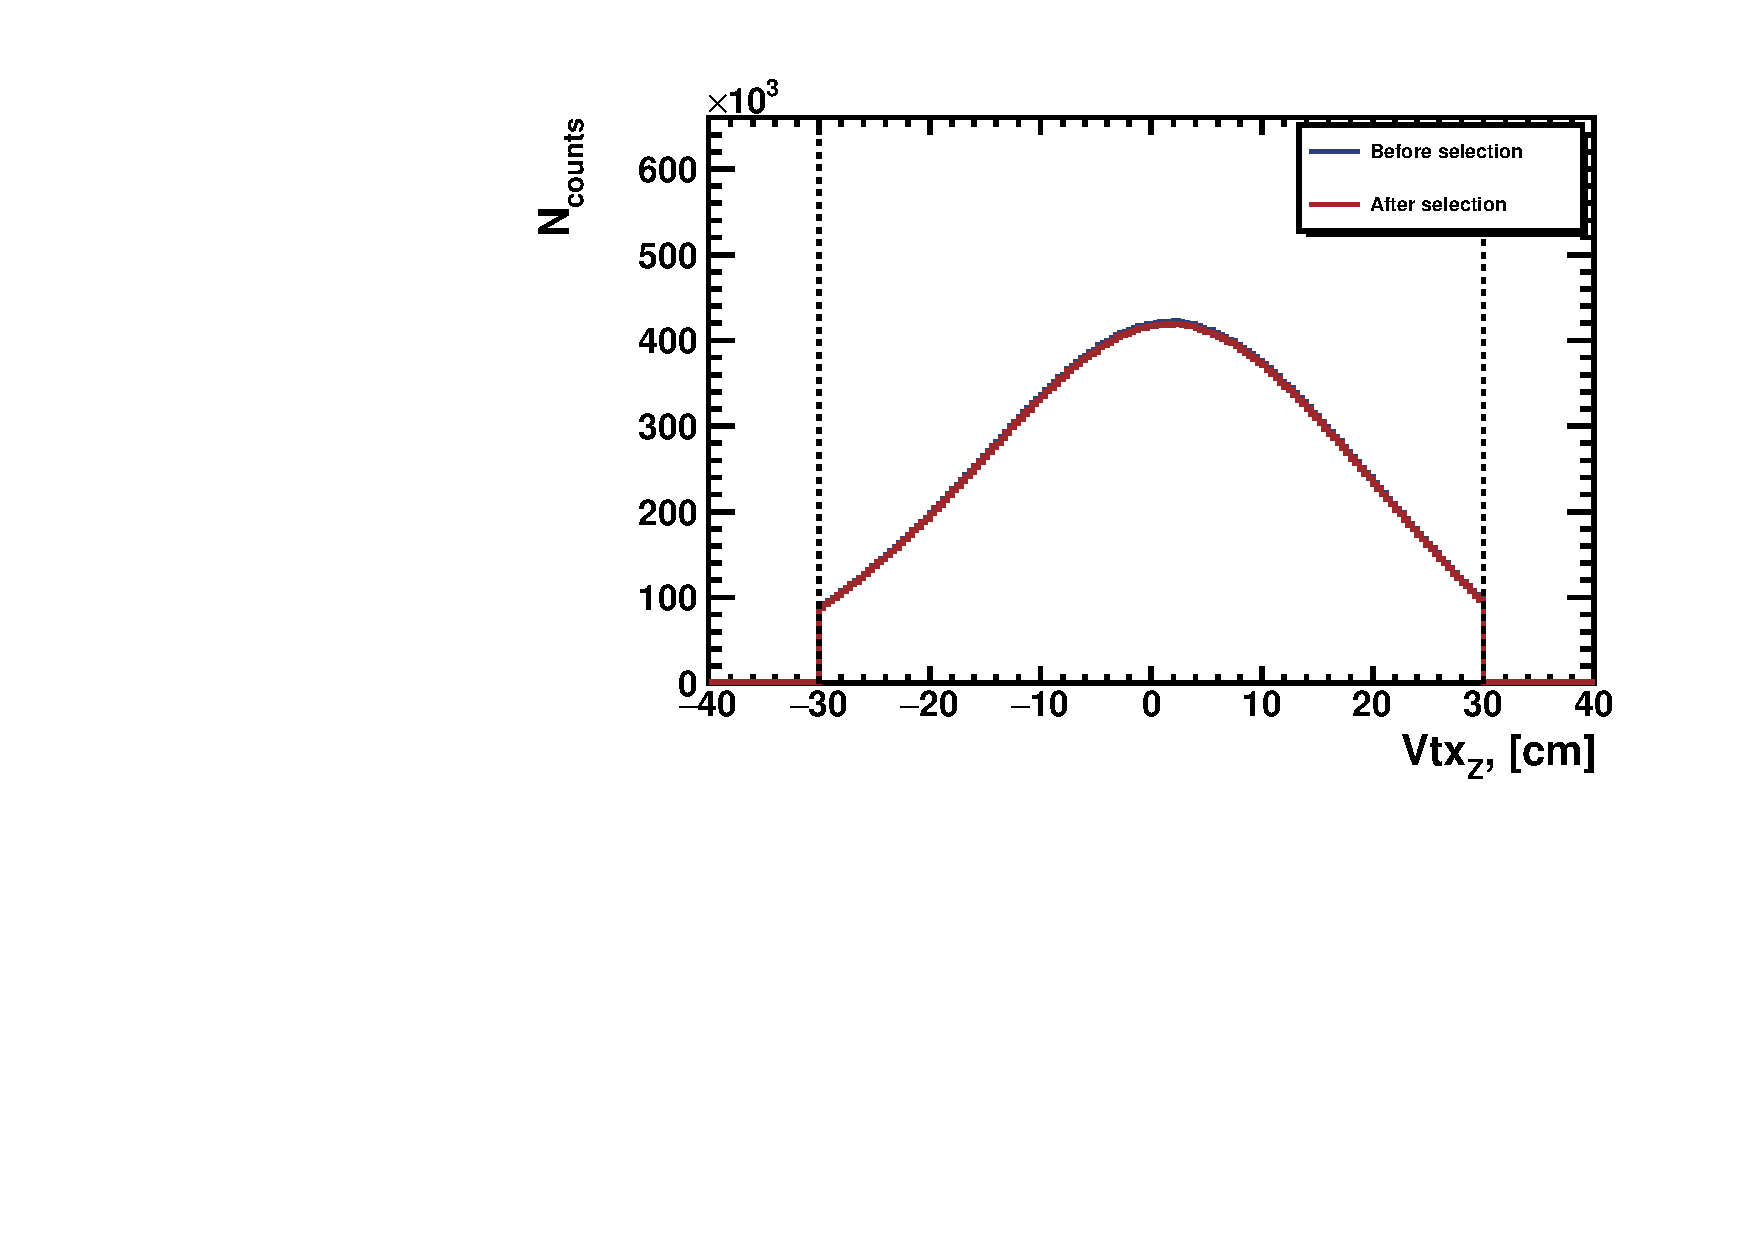
\includegraphics[width=0.49\textwidth]{Figures/VtxZ.pdf}
        \hfill
        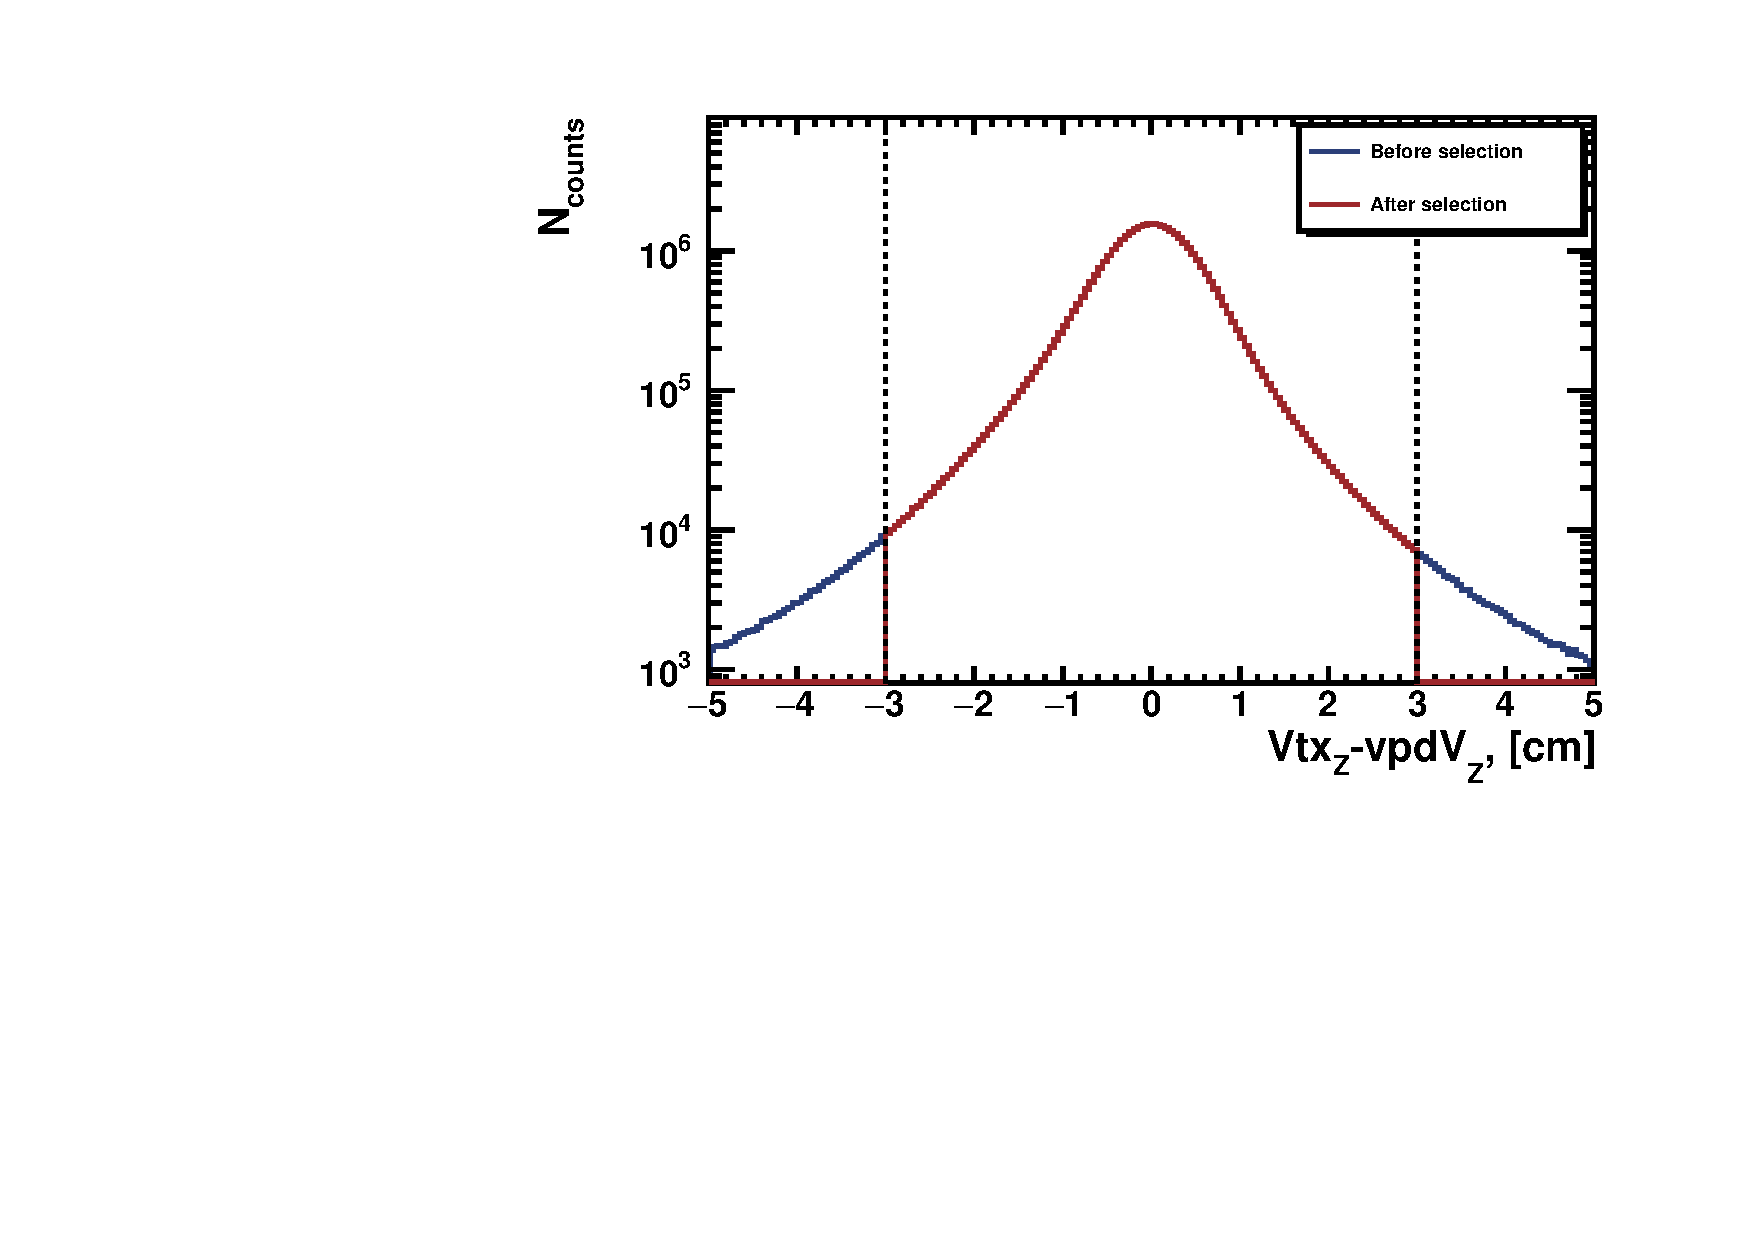
\includegraphics[width=0.49\textwidth]{Figures/VtxVpdZ.pdf}
    \end{multicols}
    \label{fig:VtxZCuts}
    \caption{Distribution of the $Vtx_Z$ (left) and $Vtx_Z - Vpd_Z$ (right).}
\end{figure}

\begin{figure}[ht]
    \begin{multicols}{2}
        \hfill
        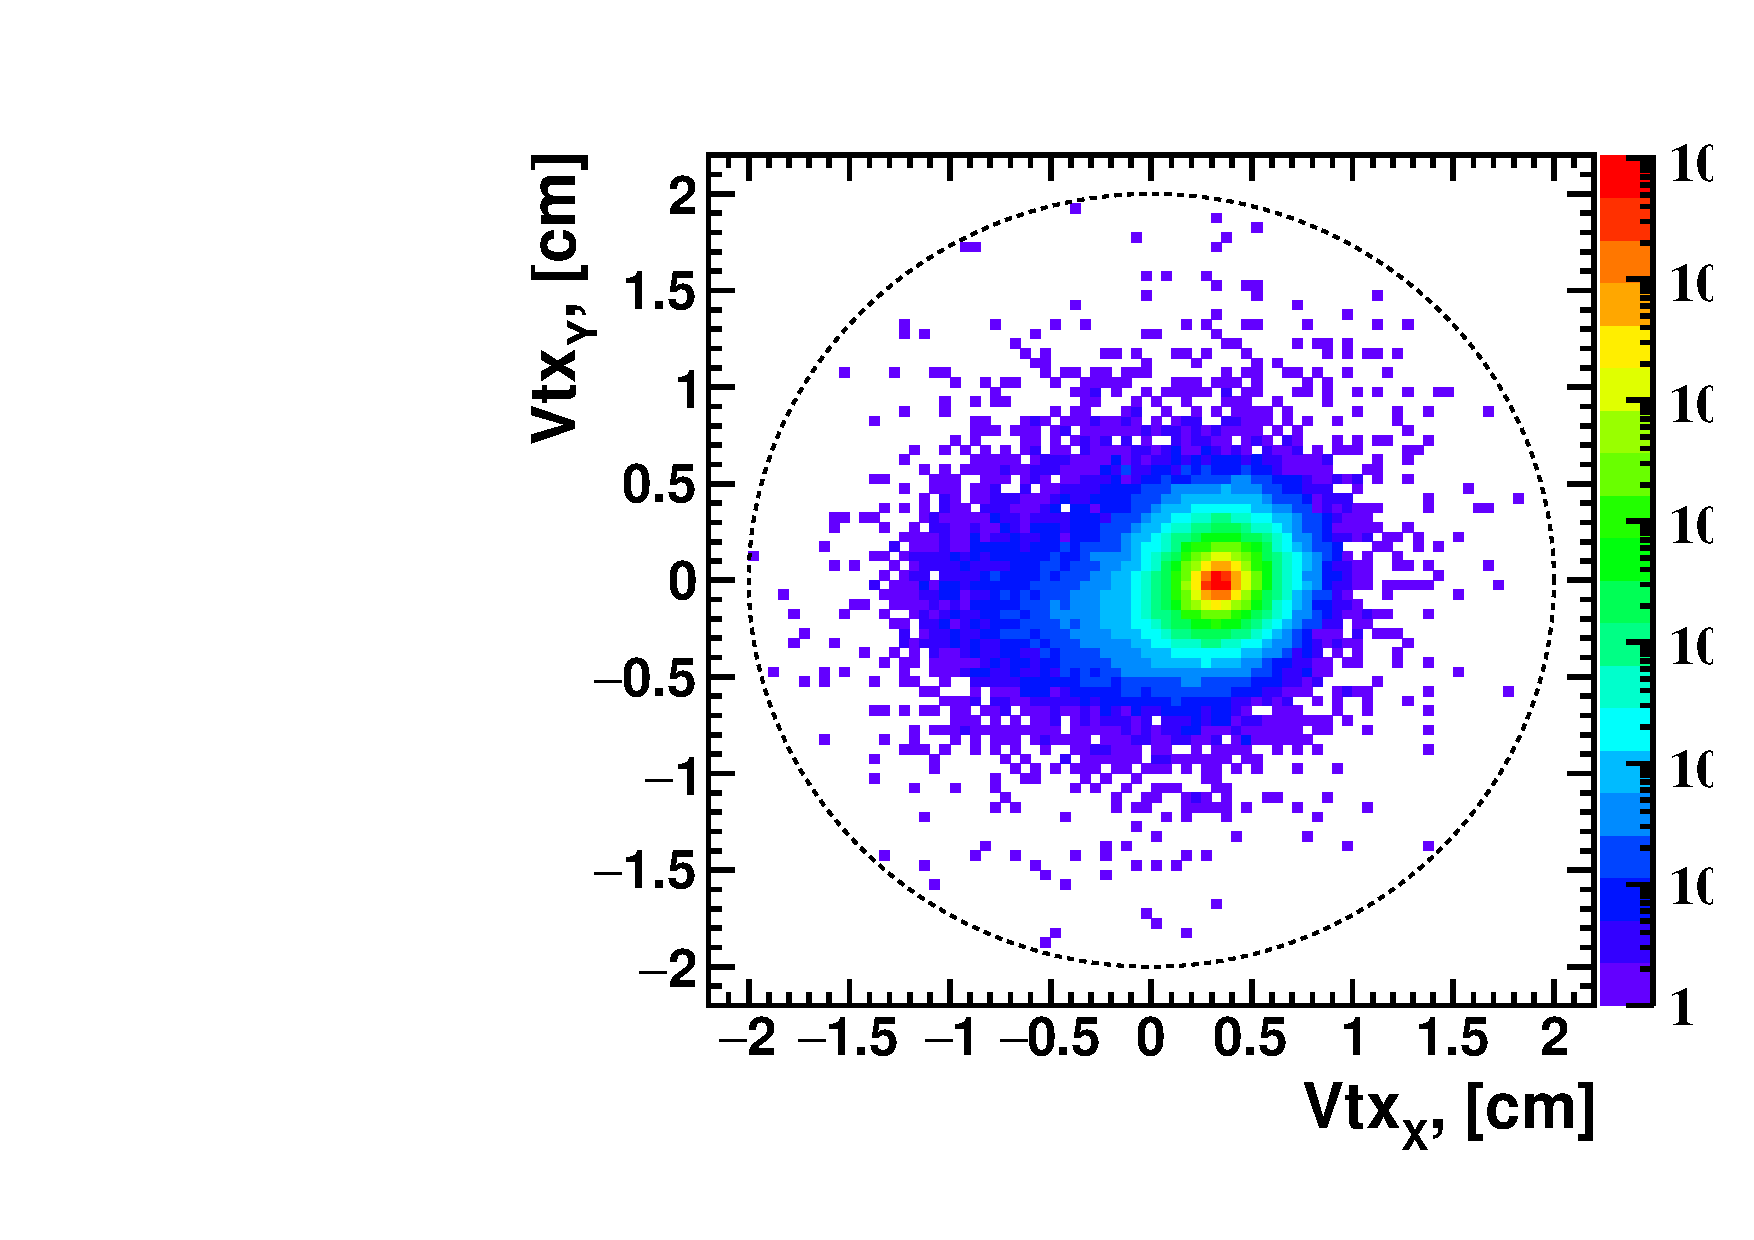
\includegraphics[width=0.49\textwidth]{Figures/VtxXY0.pdf}
        \hfill
        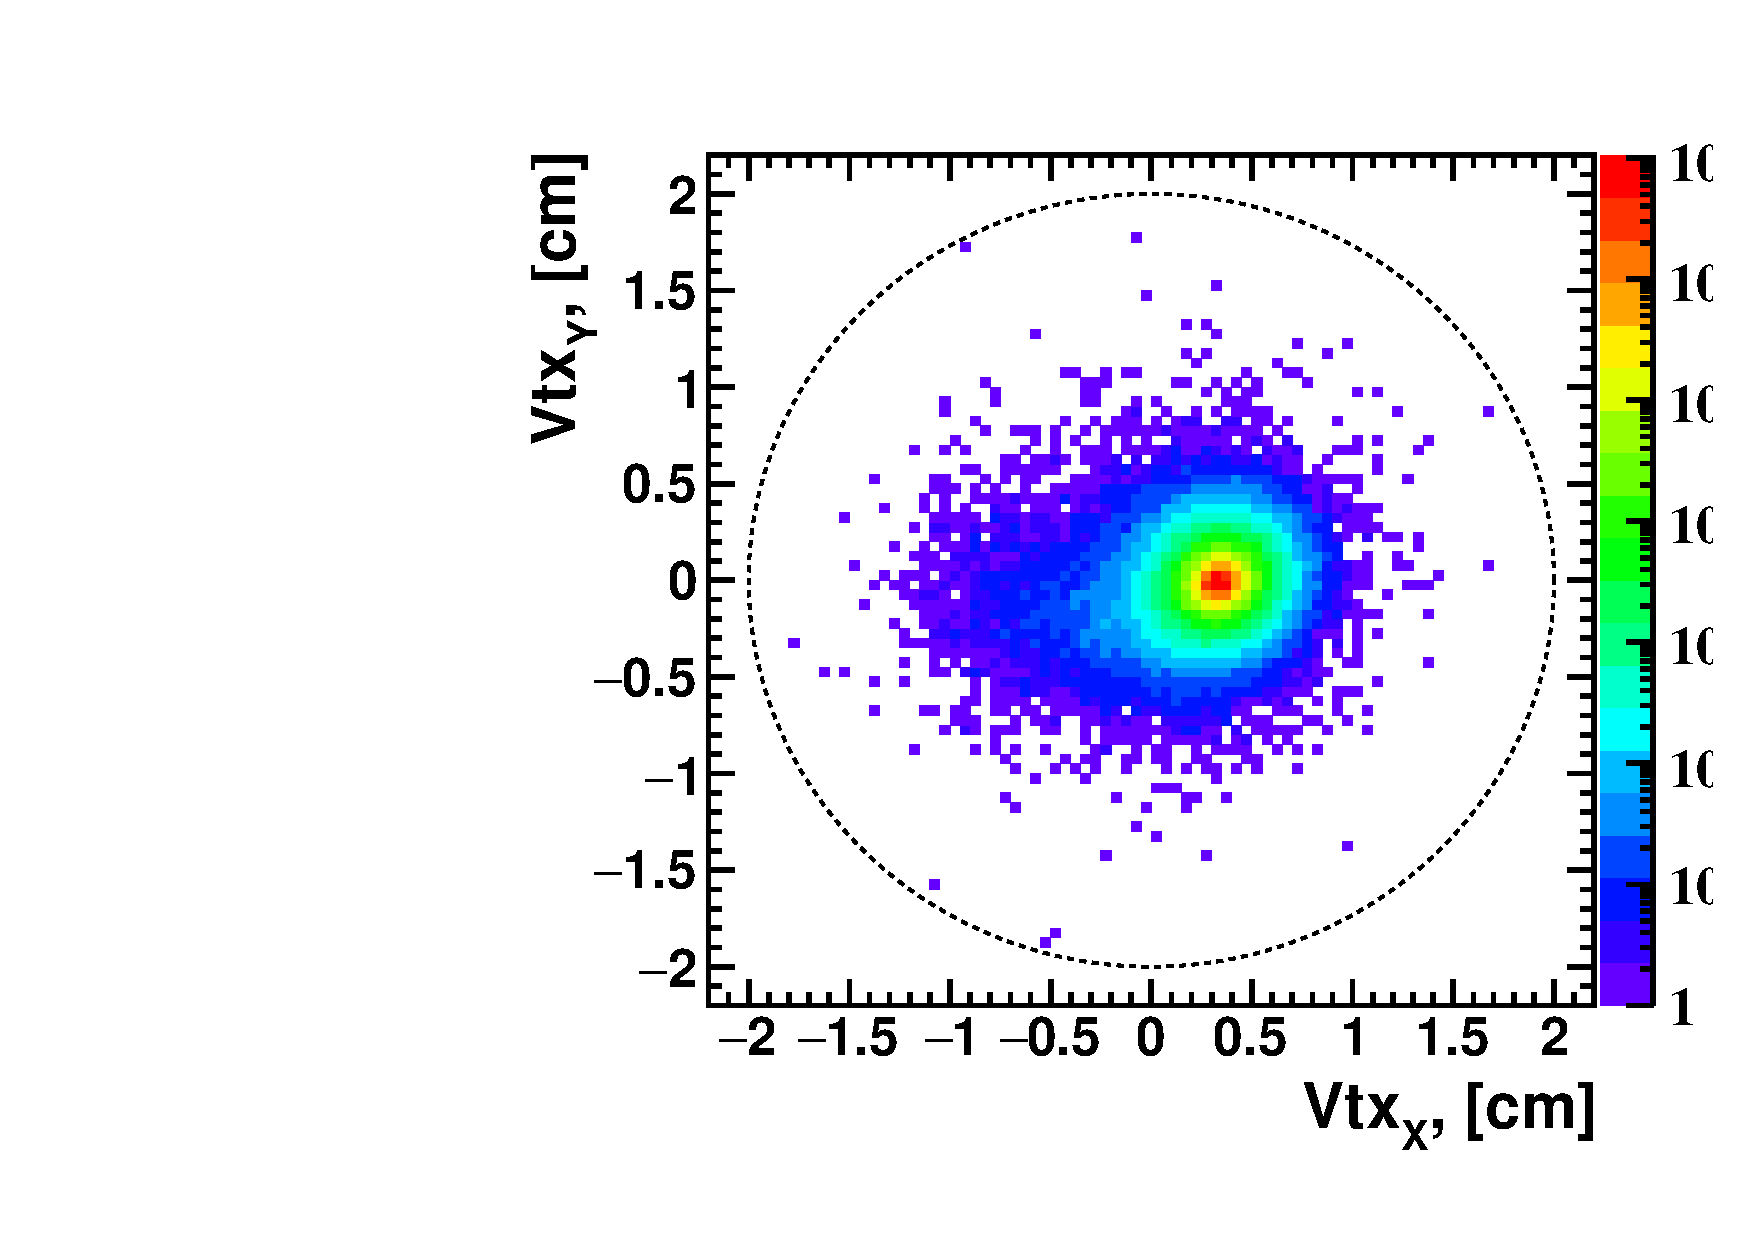
\includegraphics[width=0.49\textwidth]{Figures/VtxXY1.pdf}
    \end{multicols}
    \label{fig:VtxXYCuts}
    \caption{Distribution of the X-~and Y-components of the vertex before (left) and after (right) event selection.}
\end{figure}

\FloatBarrier
\subsection {Track selection}

\begin{figure}[ht]
    \begin{multicols}{2}
        \hfill
        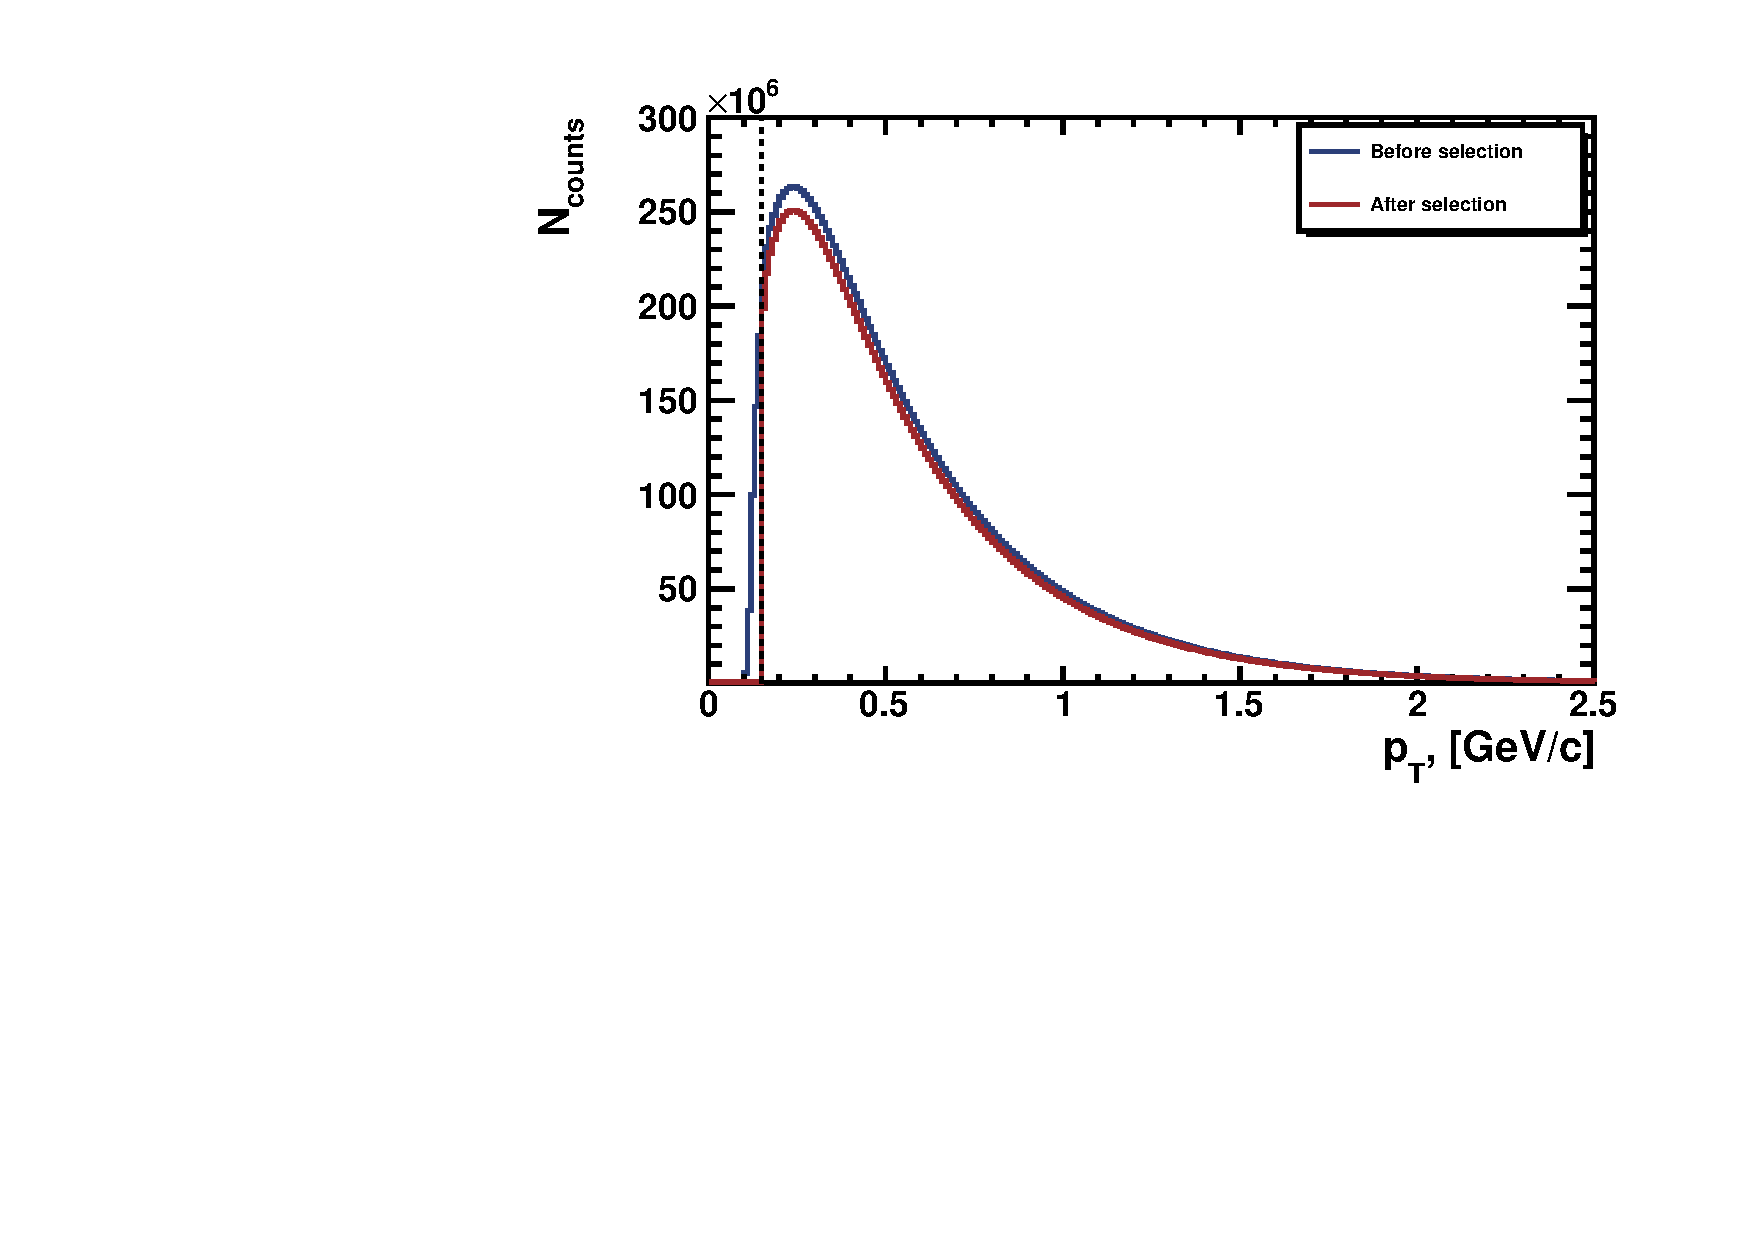
\includegraphics[width=0.49\textwidth]{Figures/Pt.pdf}
        \hfill
        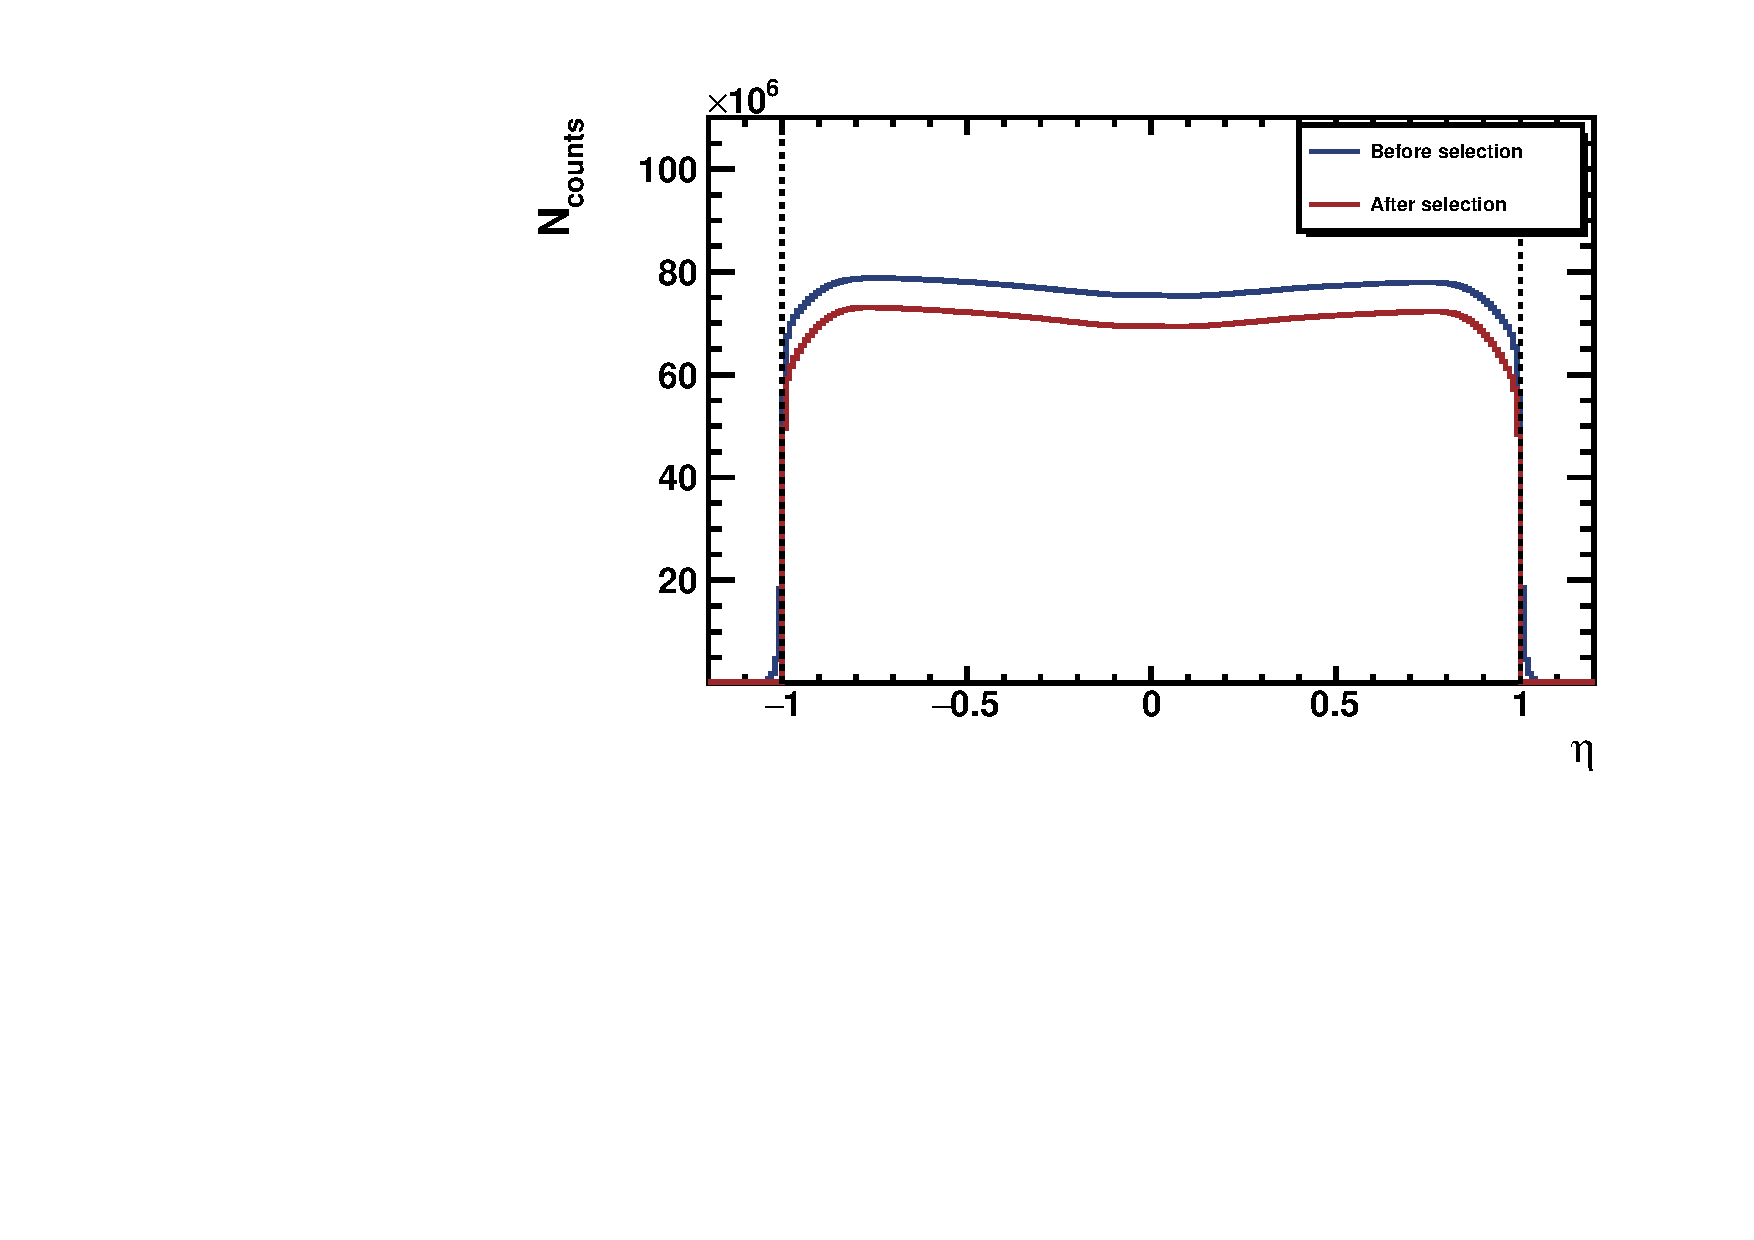
\includegraphics[width=0.49\textwidth]{Figures/Eta.pdf}
        \hfill
        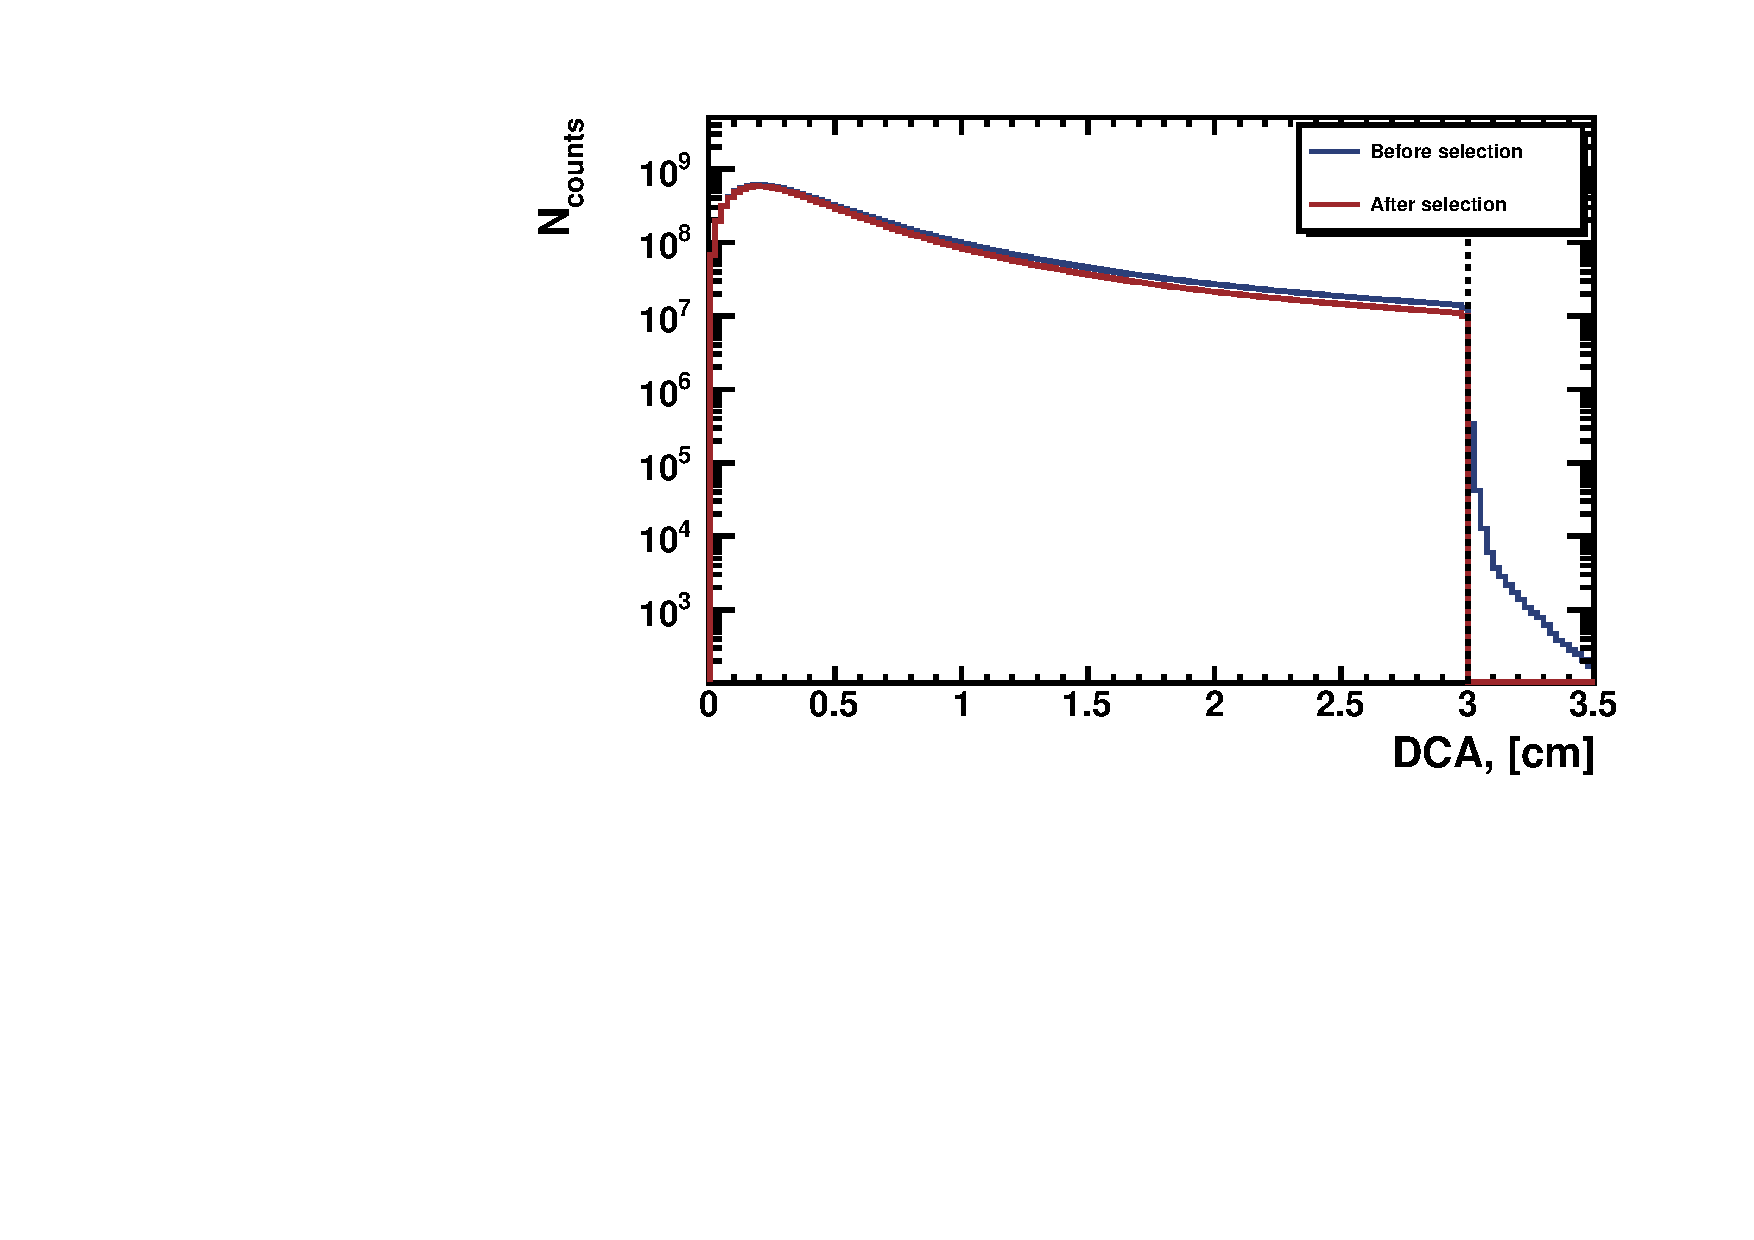
\includegraphics[width=0.49\textwidth]{Figures/DCA.pdf}
        \hfill
        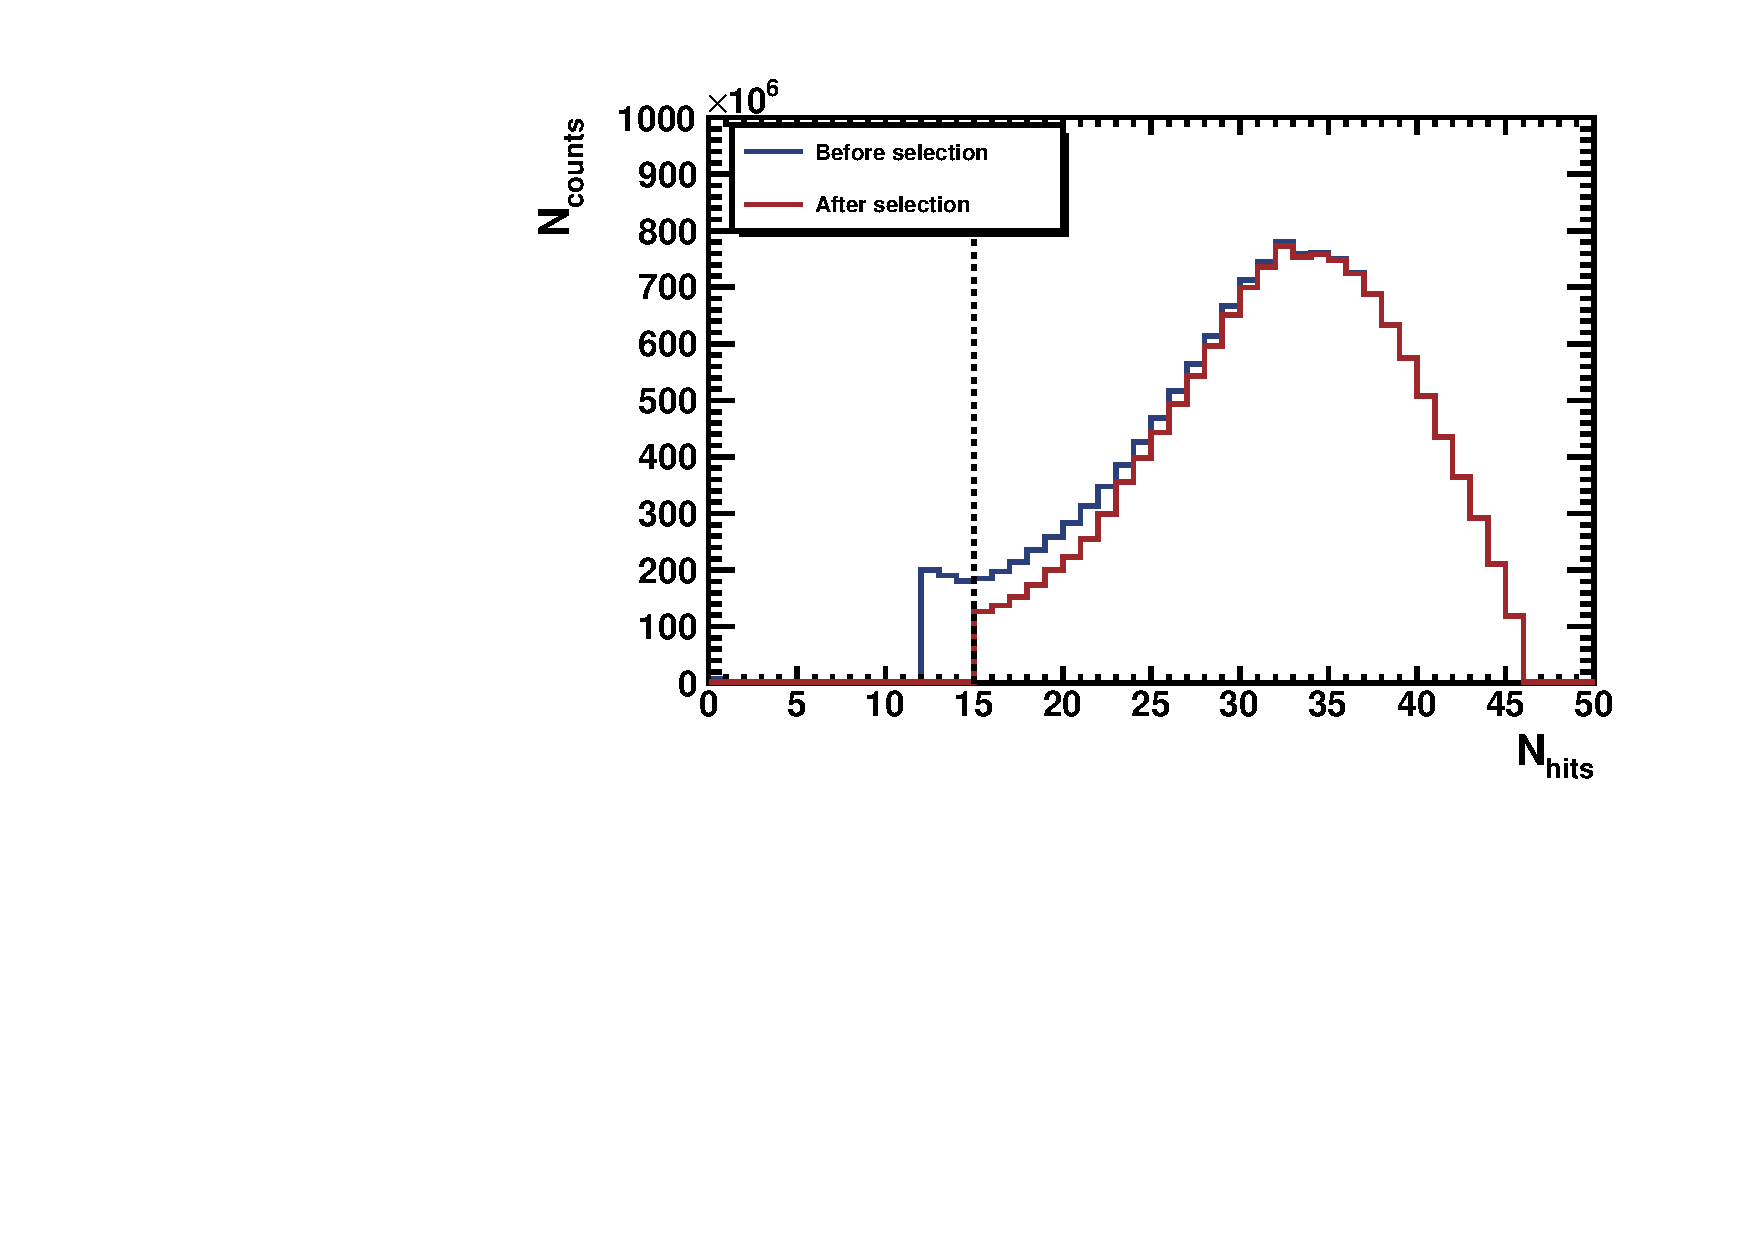
\includegraphics[width=0.49\textwidth]{Figures/Nhits.pdf}
    \end{multicols}
    \label{fig:TrackSelection}
    \caption{(upper left) $p_T$-distribution, (upper right) $|$\DCA$|$, (bottom left) $\eta$ and (bottom right) $N_{hits}$ distributions before and after track selection.}
\end{figure}

\FloatBarrier
\subsection {Particle identification}

\begin{figure}[ht]
    \begin{subfigure}{.49\textwidth}
        \centering
        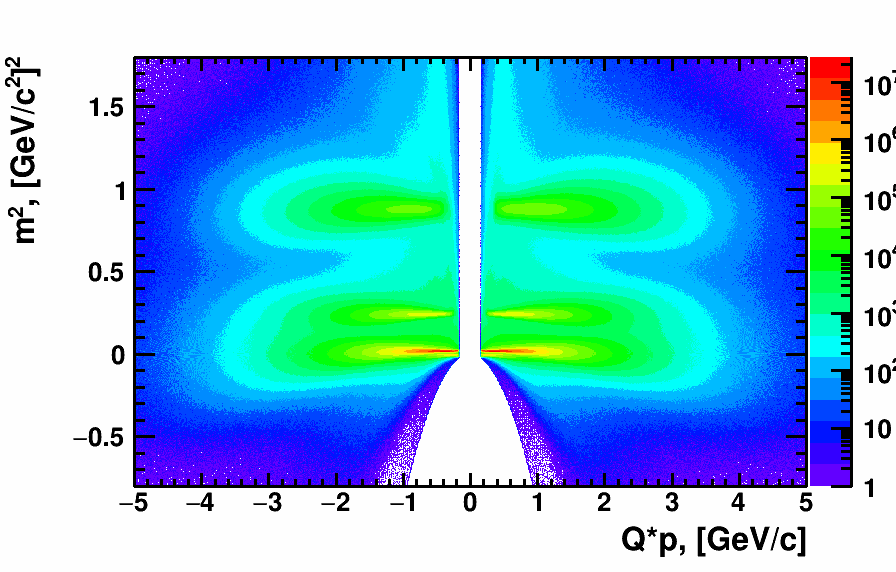
\includegraphics[width=1.\linewidth]{Figures/M2Qp_before_PID.png}
        %\caption{a}
    \end{subfigure}
    \begin{subfigure}{.49\textwidth}
        \centering
        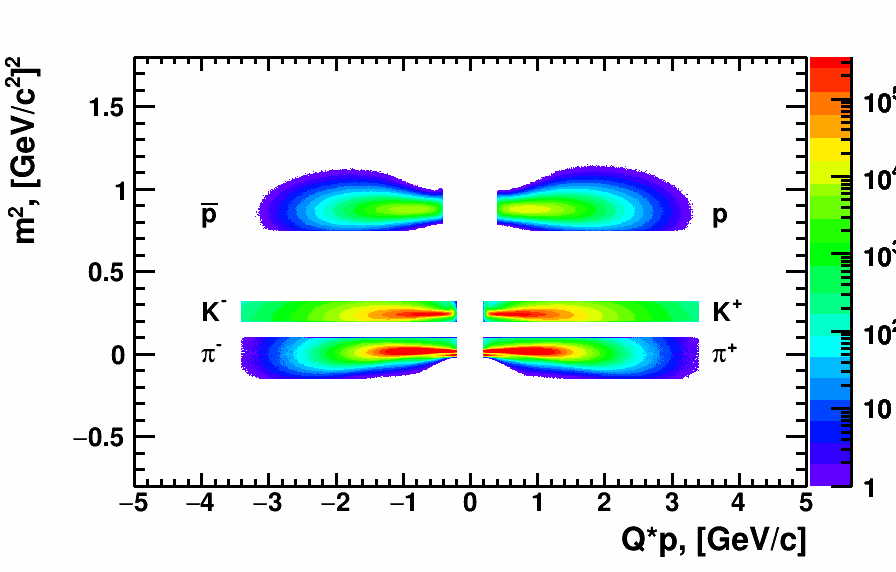
\includegraphics[width=1.\linewidth]{Figures/M2Qp_after_PID.png}
        %\caption{b}
    \end{subfigure}
    \label{fig:M2vsQp}
    \caption{$m^2$ estimated using \TPC\ and \TOF\ detectors vs charged total momentum $Q\cdot p$ before (left) and after (right) \PID\ procedure.}
\end{figure}
%\newpage
%\section{Getting Started}
%\input{getstart.tex}


%\chapter*{}
\FloatBarrier
\section{Flow methods}
\subsection{The event-plane method}

\subsubsection{\TPC\ event plane}

\subsubsection{\BBC\ event plane}

\subsection{The scalar product method}

%\chapter*{}
\FloatBarrier
\section{Results \& Discussions}
\FloatBarrier
\subsection{The event-plane resolution}

\begin{figure}[ht]
    \centering
    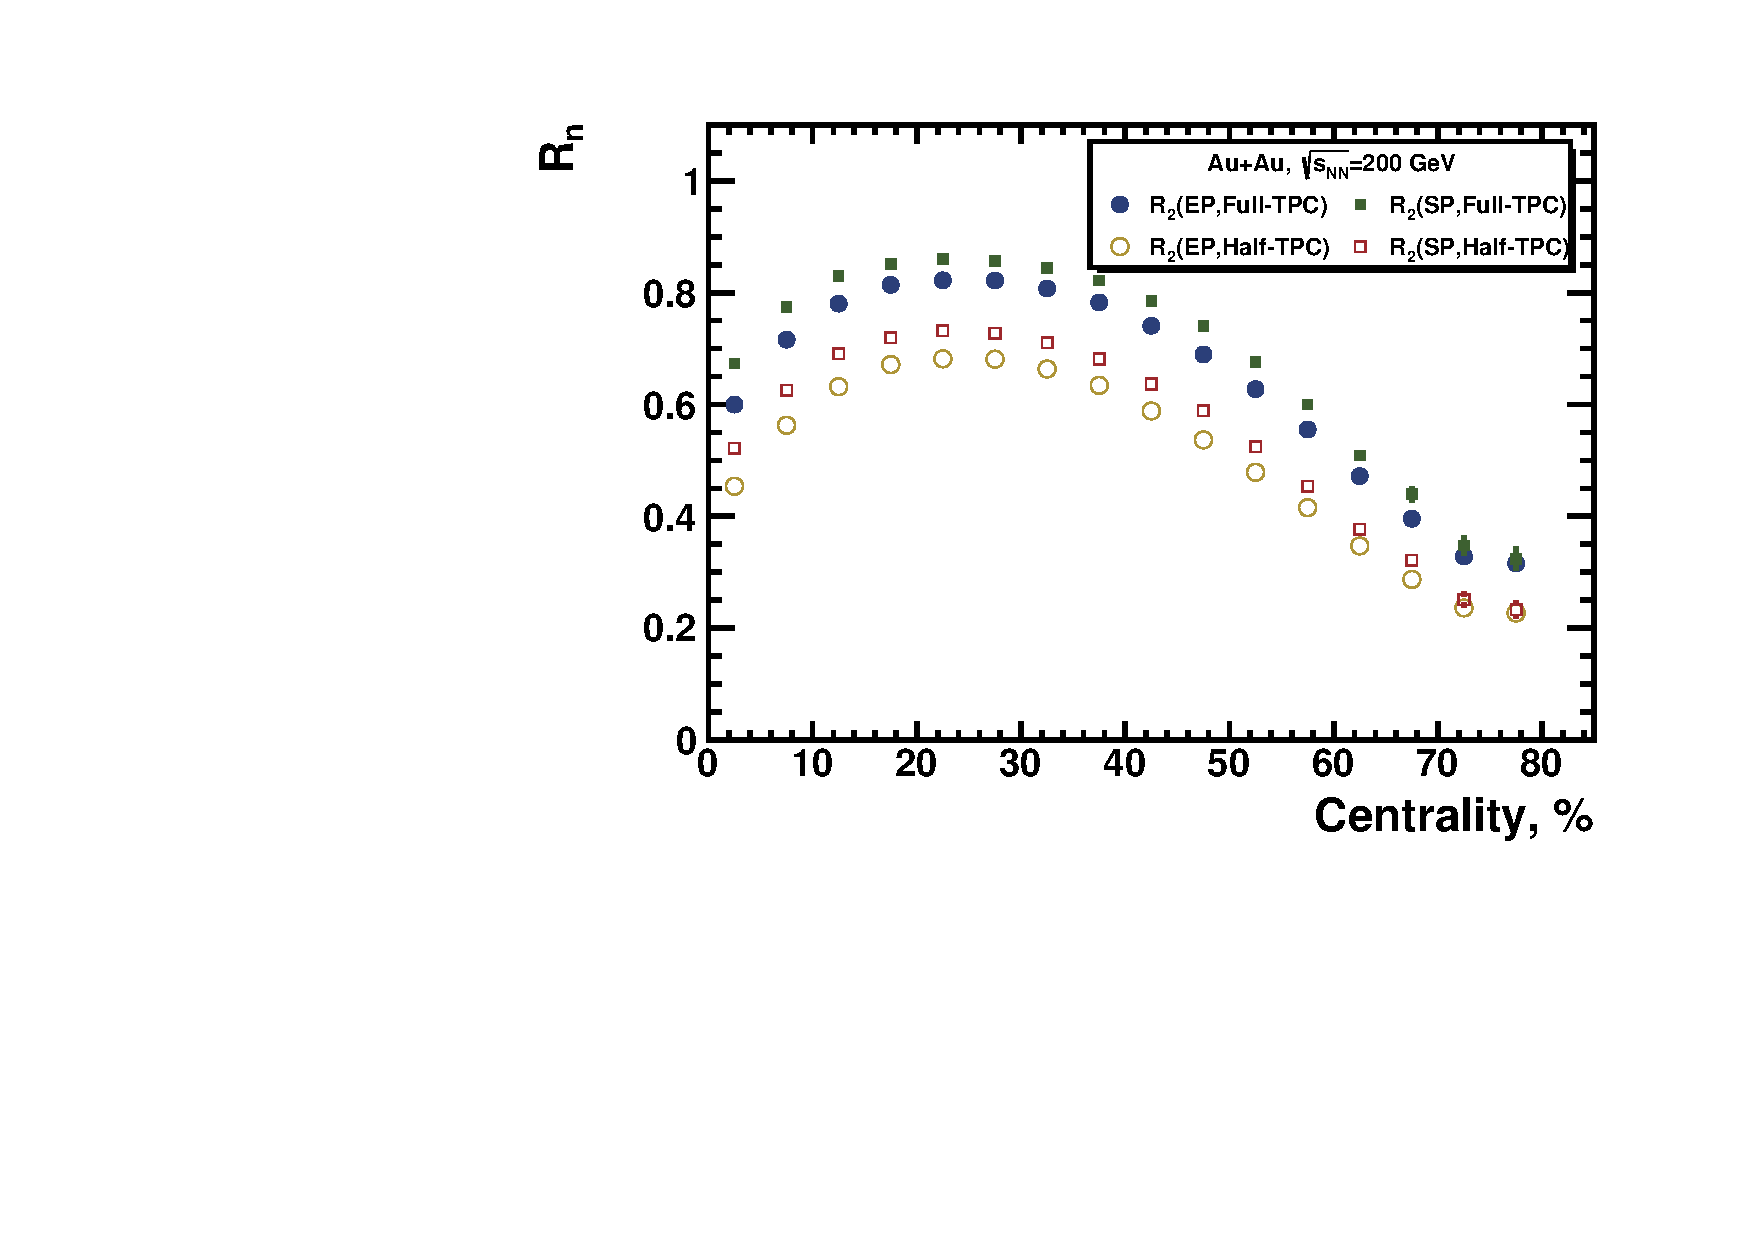
\includegraphics[width=0.7\linewidth]{Figures/ResSPFullHalfvn.pdf}
    \caption{Resolution correction factor}
    \label{fig:res_SP}
\end{figure}

\FloatBarrier
\subsection{$p_{T}$-dependence of $v_2$ \& $v_3$}

\FloatBarrier
\subsection{Method comparison}

\FloatBarrier
\section{Appendix}
\FloatBarrier
\subsection{Run-by-run check}

\begin{figure}[ht]
    \begin{subfigure}{.49\textwidth}
        \centering
        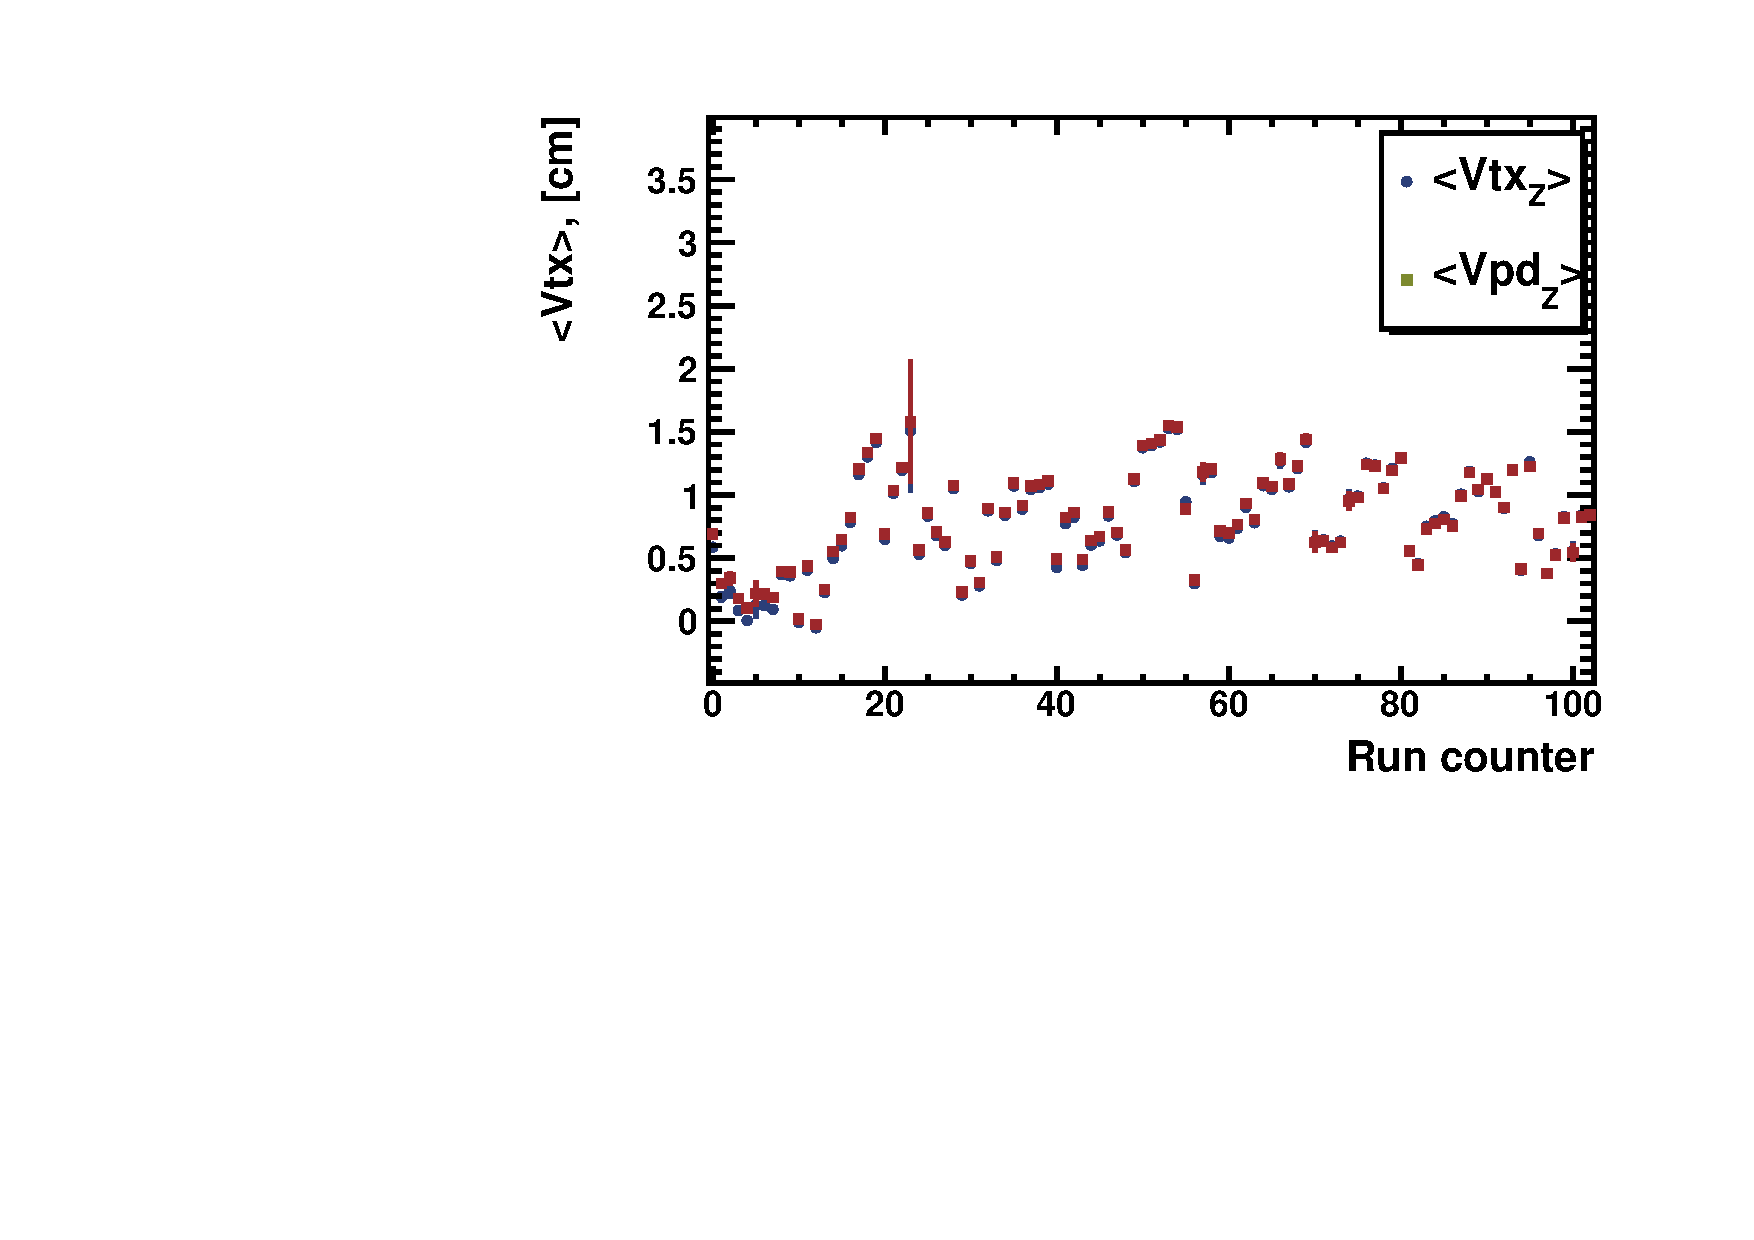
\includegraphics[width=1.\linewidth]{Figures/VtxZVsRun.pdf}
        %\caption{a}
    \end{subfigure}
    \begin{subfigure}{.49\textwidth}
        \centering
        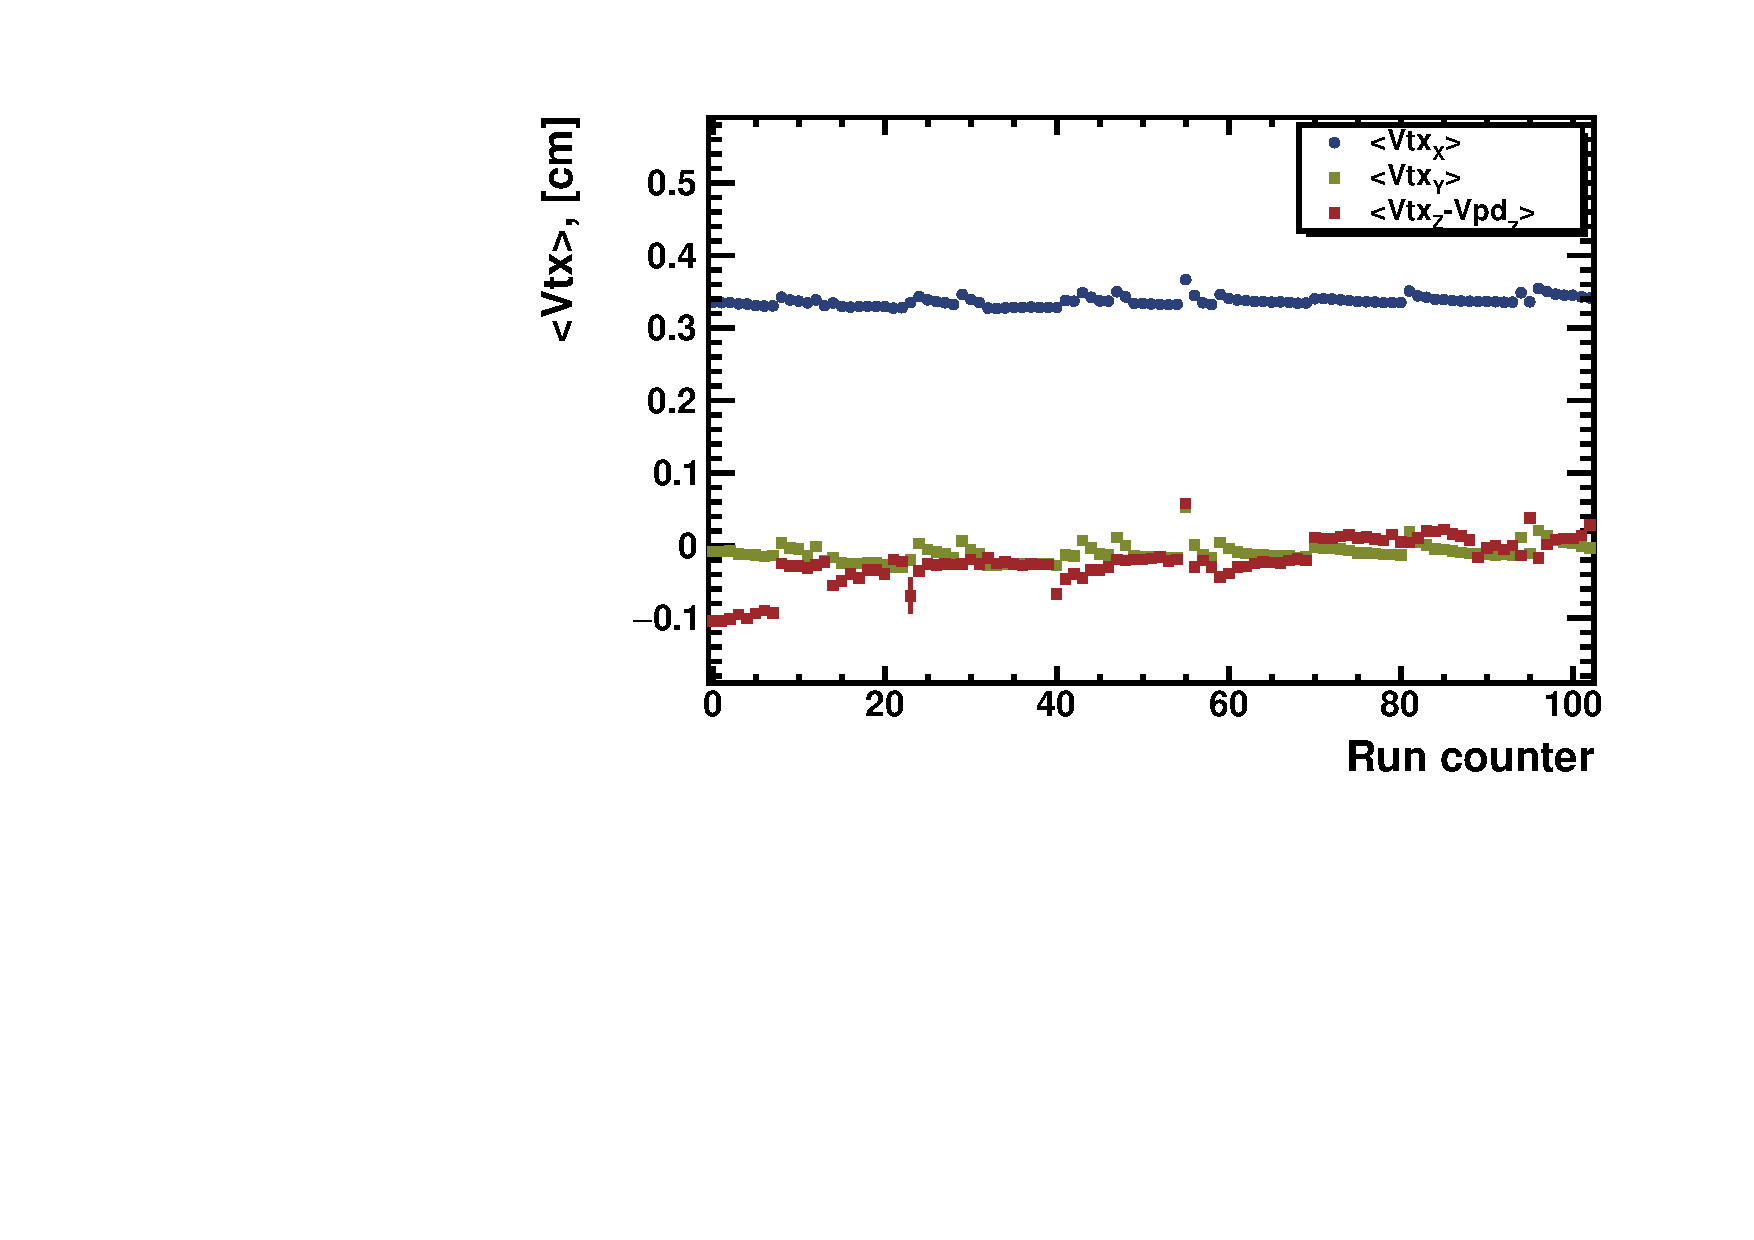
\includegraphics[width=1.\linewidth]{Figures/VtxXYVsRun.pdf}
        %\caption{b}
    \end{subfigure}
    \label{fig:VtxVsRun}
    \caption{Distributions of the $Vtx_Z$, $Vpd_Z$ (left) and $Vpd_X$, $Vpd_Y$, $Vtx_Z - Vpd_Z$ (right) as a function of run.}
\end{figure}

\begin{figure}[ht]
    \begin{subfigure}{.49\textwidth}
        \centering
        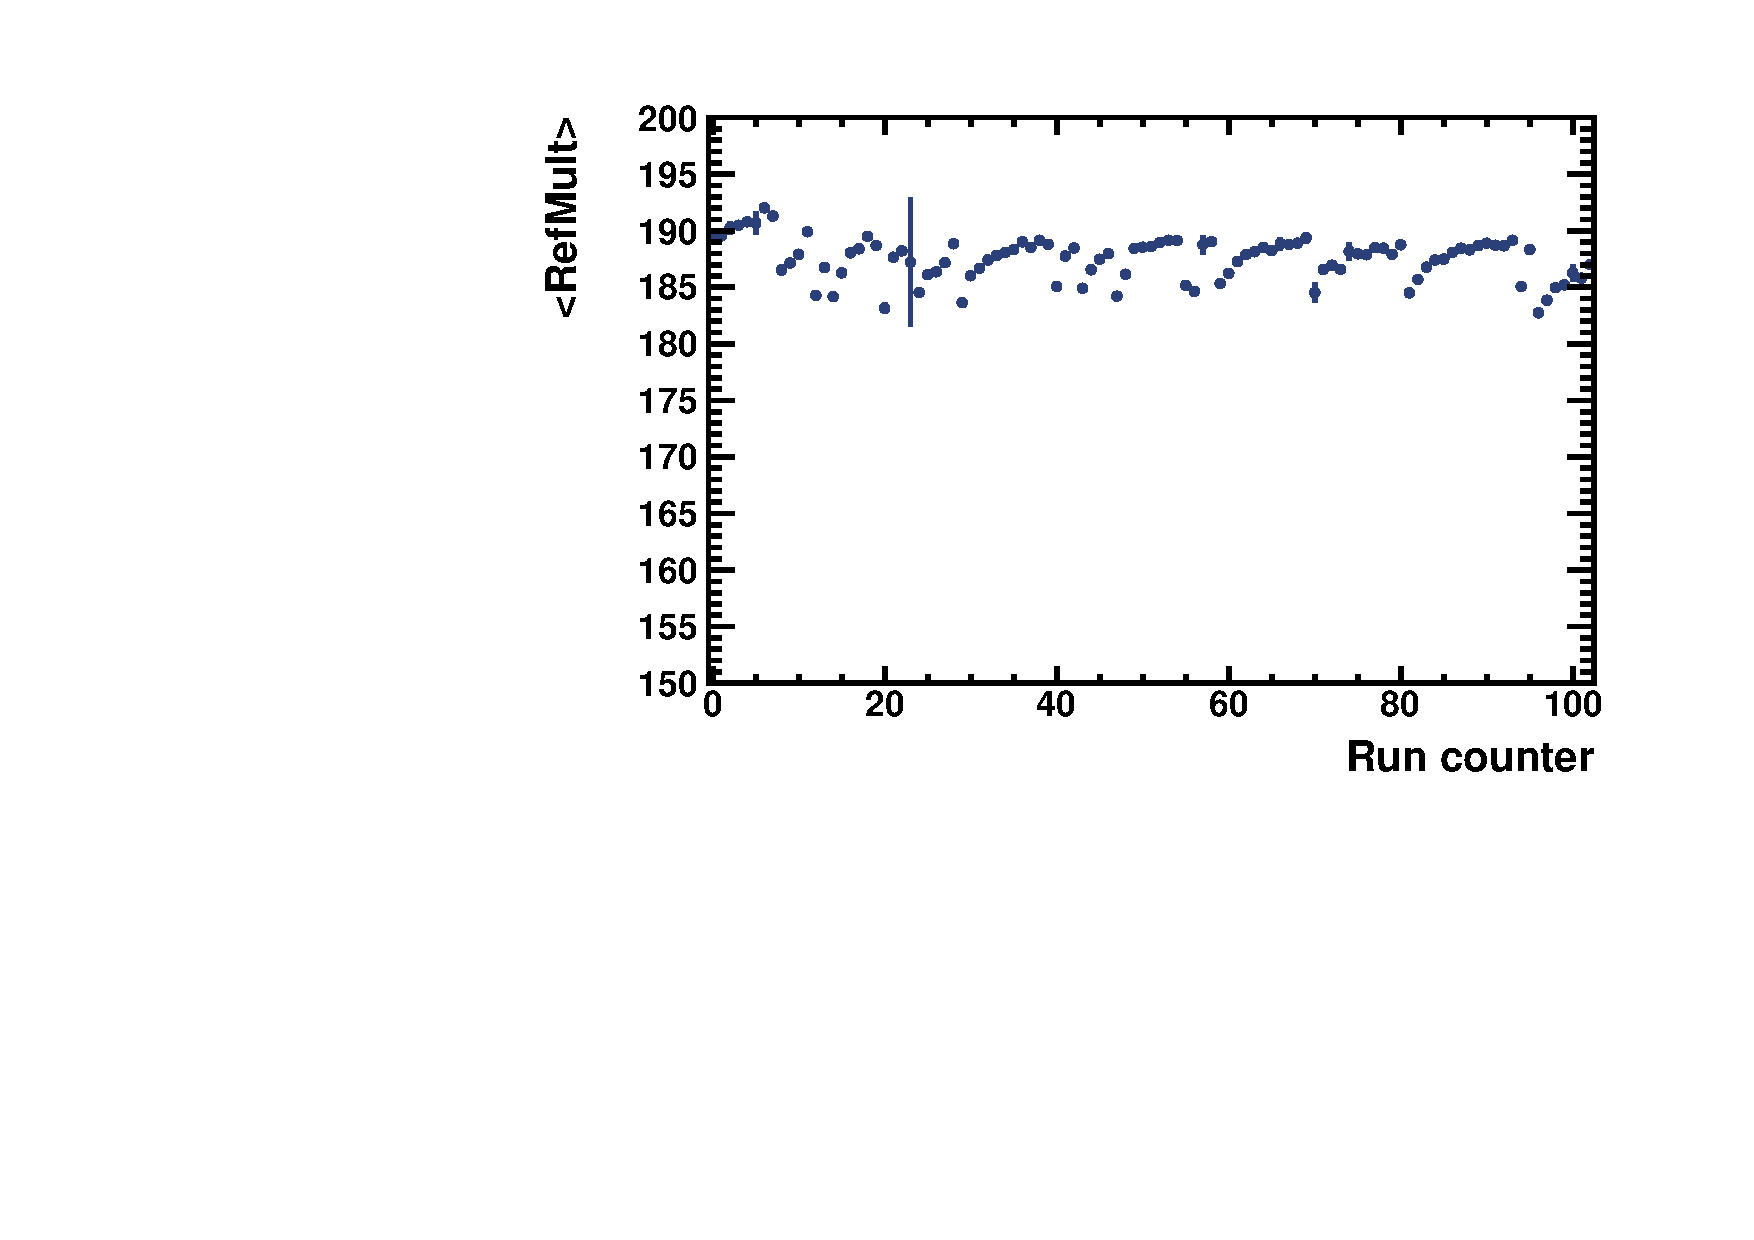
\includegraphics[width=1.\linewidth]{Figures/RefMultVsRun.pdf}
        %\caption{a}
    \end{subfigure}
    \begin{subfigure}{.49\textwidth}
        \centering
        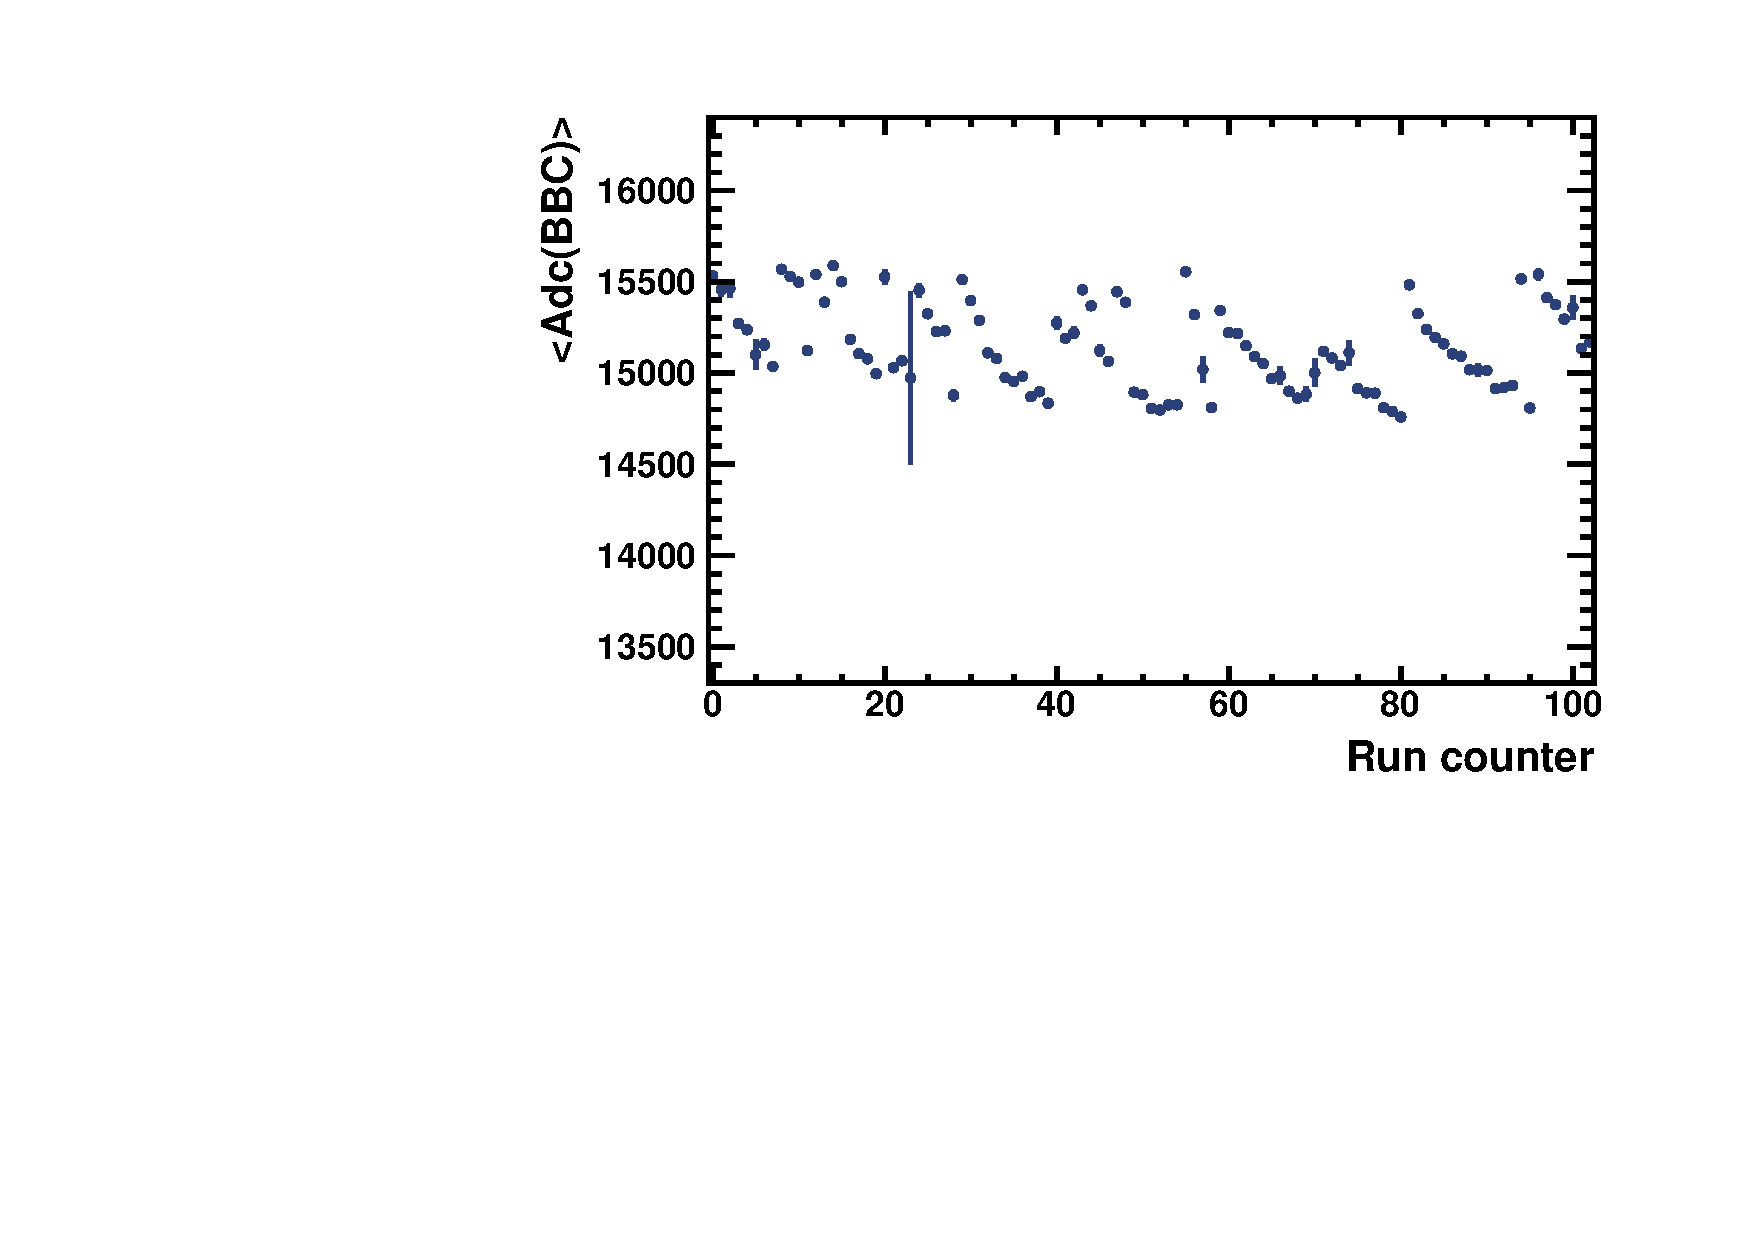
\includegraphics[width=1.\linewidth]{Figures/AdcVsRun.pdf}
        %\caption{b}
    \end{subfigure}
    \label{fig:RefMultAdcVsRun}
    \caption{Distributions of the RefMult (left) and Adc from \BBC\ (right) as a function of run.}
\end{figure}

\begin{figure}[ht]
    \begin{subfigure}{.49\textwidth}
        \centering
        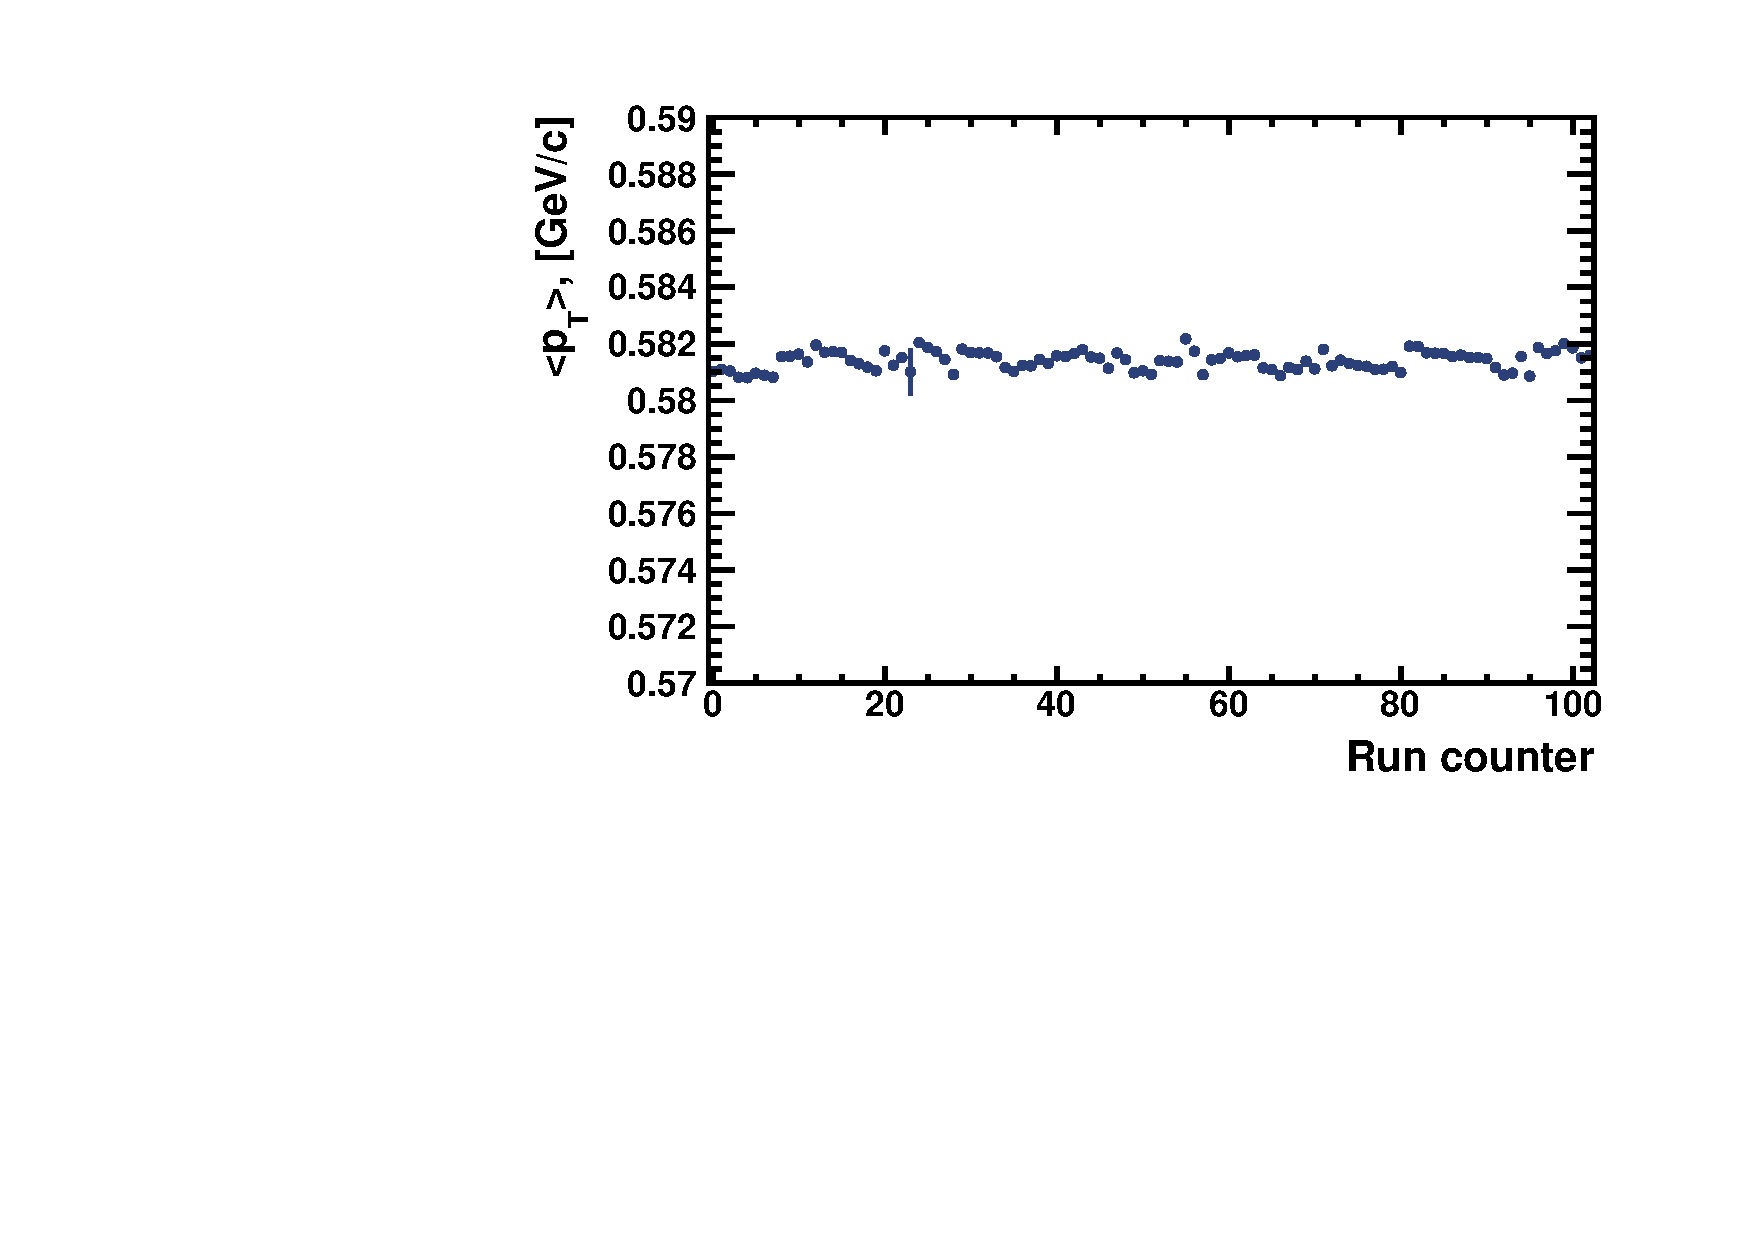
\includegraphics[width=1.\linewidth]{Figures/PtVsRun.pdf}
        %\caption{a}
    \end{subfigure}
    \begin{subfigure}{.49\textwidth}
        \centering
        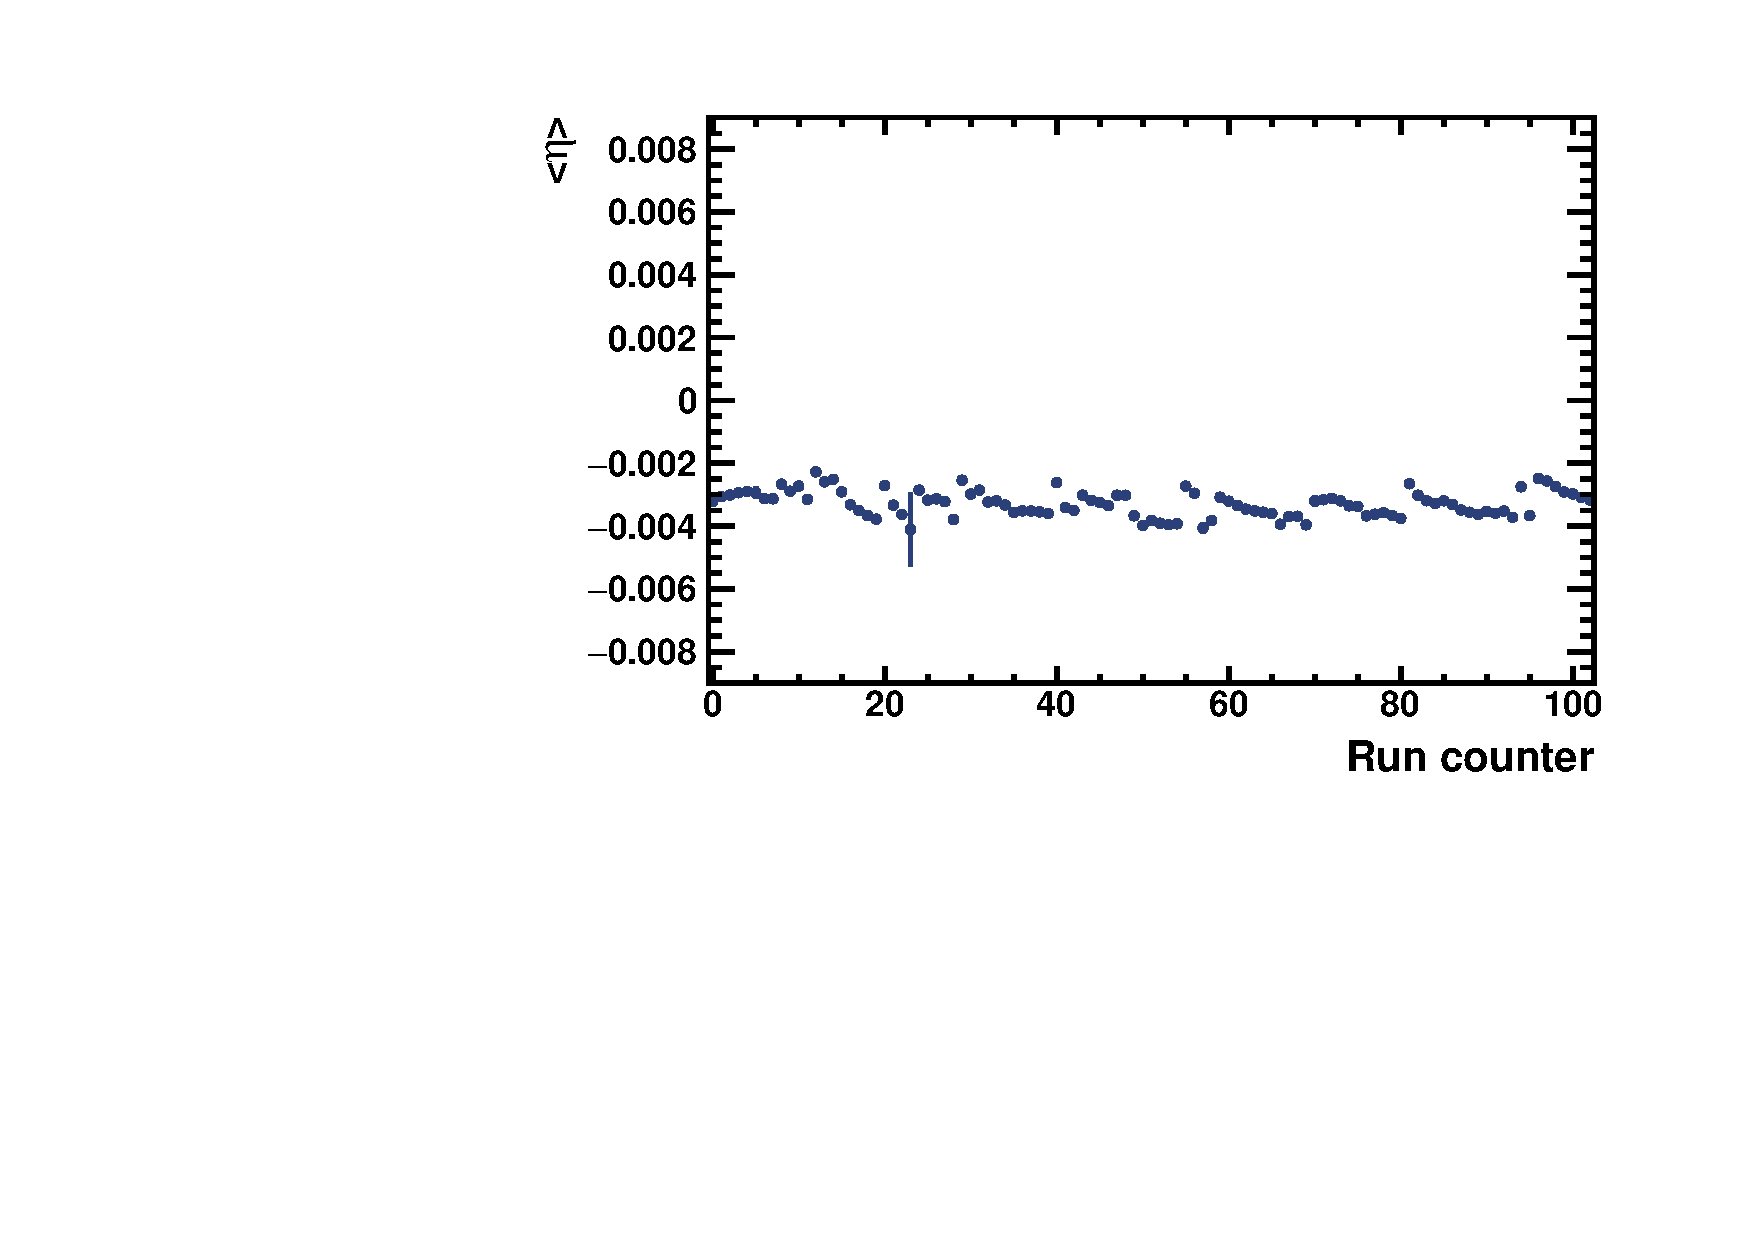
\includegraphics[width=1.\linewidth]{Figures/EtaVsRun.pdf}
        %\caption{b}
    \end{subfigure}
    \\
    \begin{subfigure}{.49\textwidth}
        \centering
        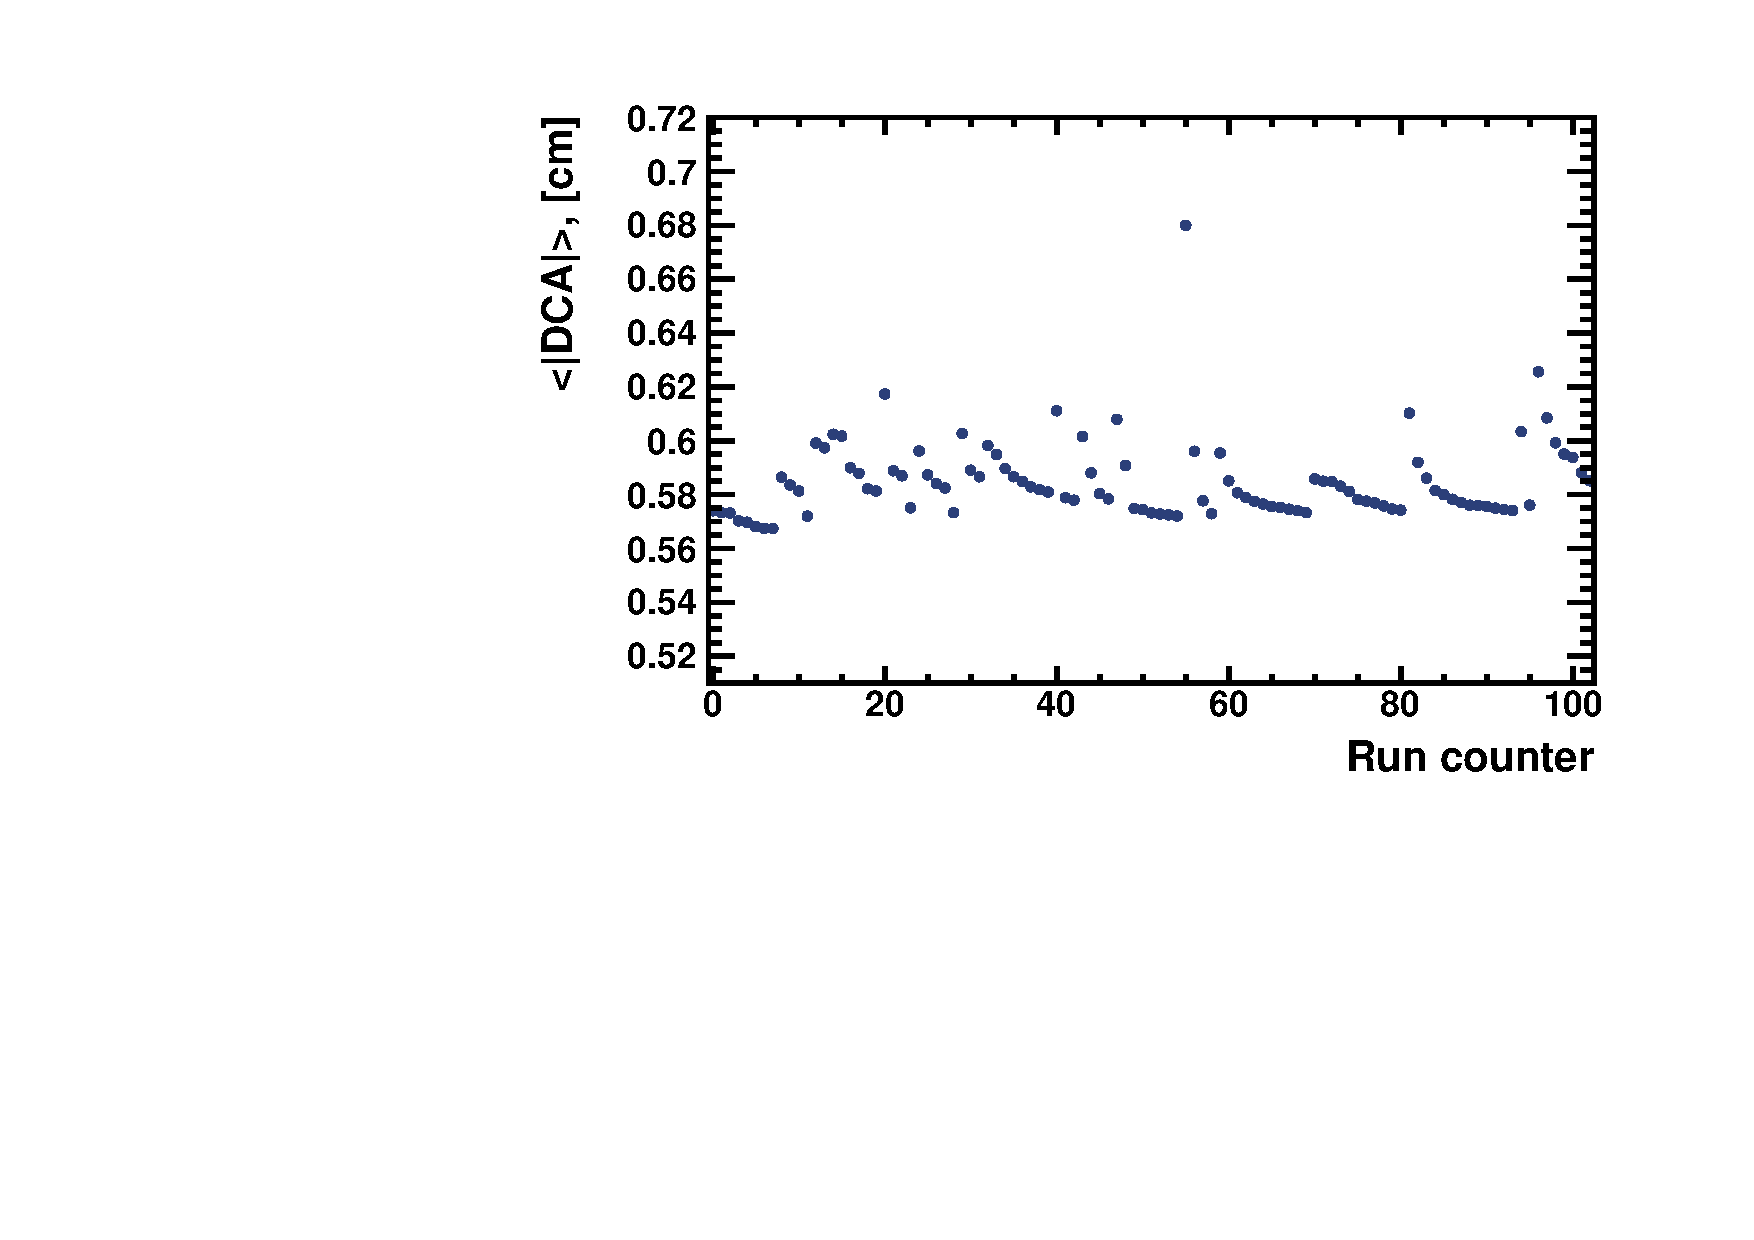
\includegraphics[width=1.\linewidth]{Figures/DCAVsRun.pdf}
        %\caption{a}
    \end{subfigure}
    \begin{subfigure}{.49\textwidth}
        \centering
        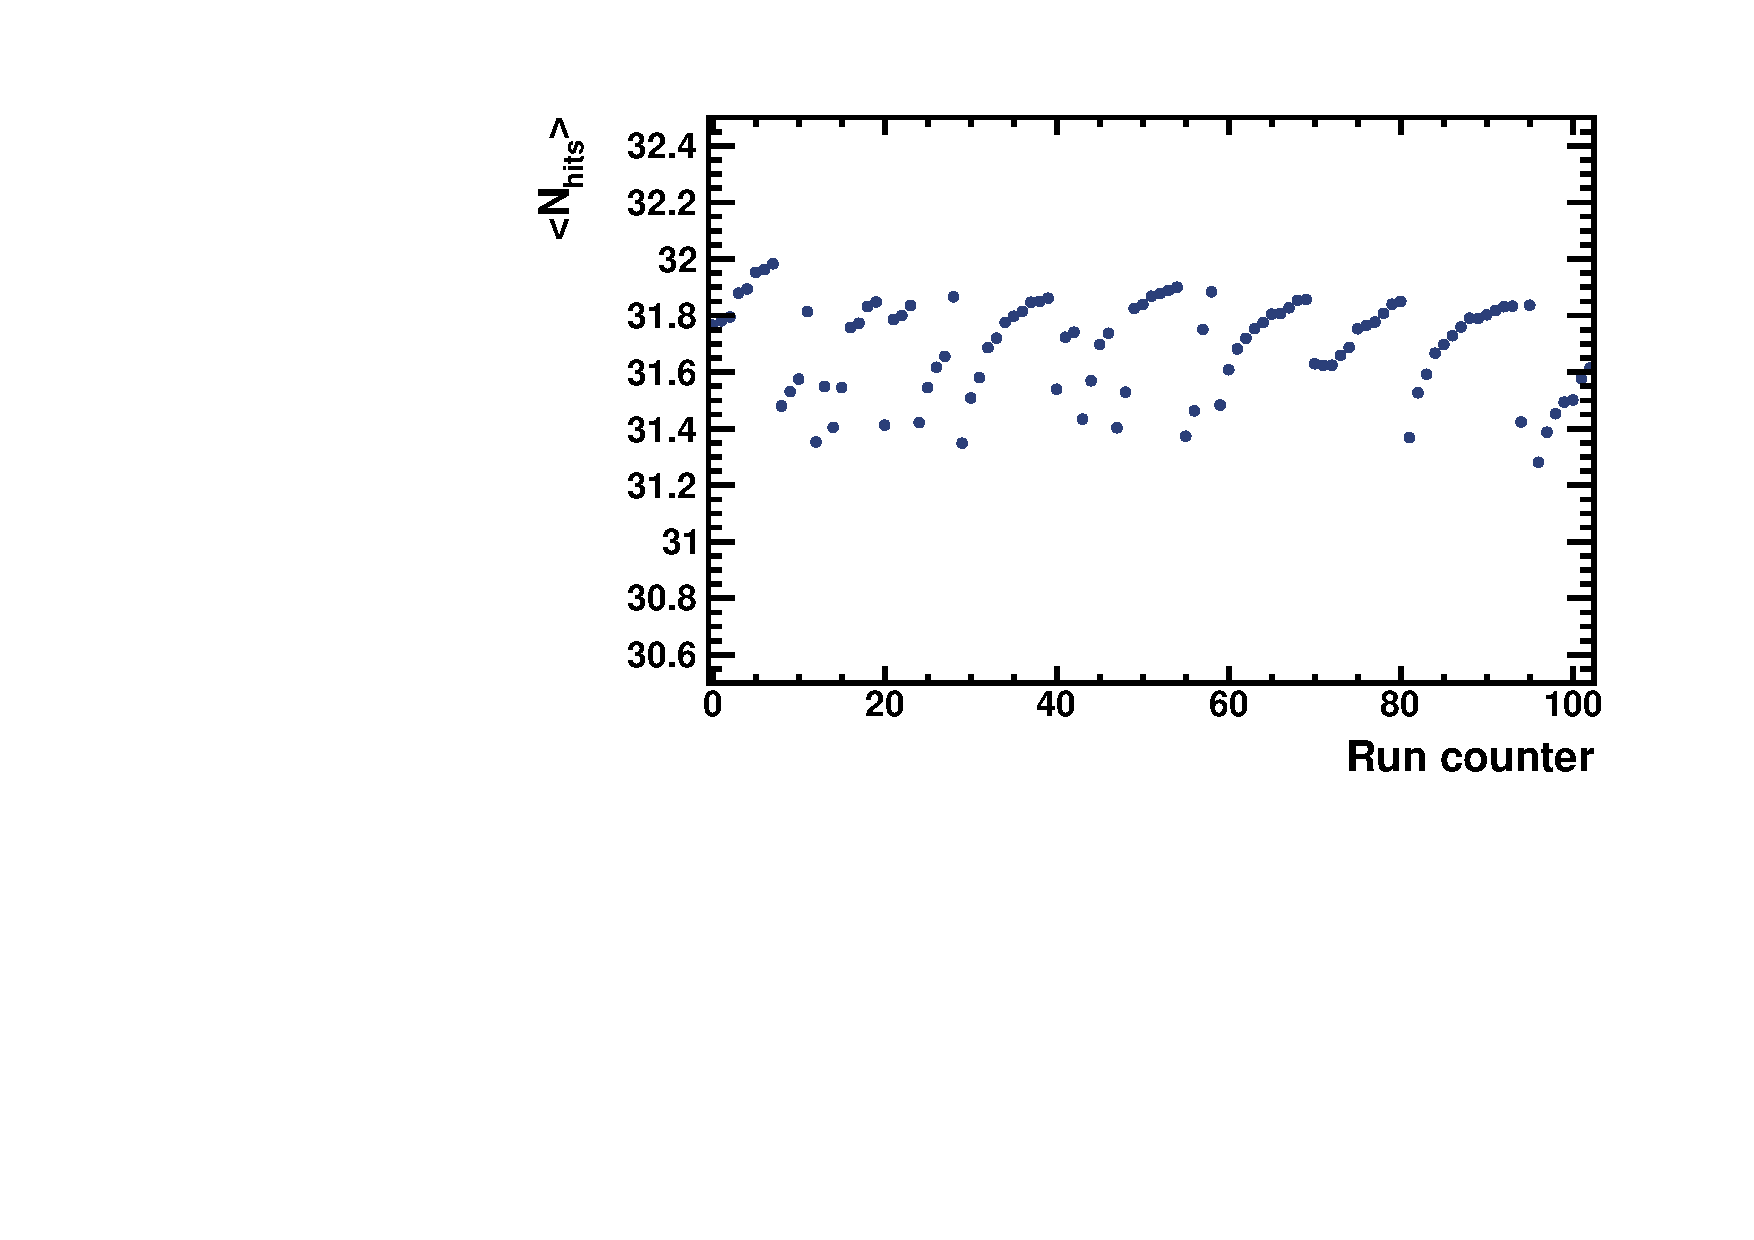
\includegraphics[width=1.\linewidth]{Figures/NhitsFitVsRun.pdf}
        %\caption{b}
    \end{subfigure}
    \label{fig:TrackVsRun}
    \caption{Distributions of the $p_{T}$ (upper left), $\eta$ (upper right), \DCA\ (bottom left) and $N_{hits}$ (bottom right) as a function of run.}
\end{figure}

%-------------------------------------------------------------------------------
% REFERENCES
%-------------------------------------------------------------------------------
\newpage
%\section*{References}

\bibliographystyle{ieeetr}
\bibliography{References}

}
\end{document}

%-------------------------------------------------------------------------------
% SNIPPETS
%-------------------------------------------------------------------------------

%\begin{figure}[!ht]
%	\centering
%	\includegraphics[width=0.8\textwidth]{file_name}
%	\caption{}
%	\centering
%	\label{label:file_name}
%\end{figure}

%\begin{figure}[!ht]
%	\centering
%	\includegraphics[width=0.8\textwidth]{graph}
%	\caption{Blood pressure ranges and associated level of hypertension (American Heart Association, 2013).}
%	\centering
%	\label{label:graph}
%\end{figure}

%\begin{wrapfigure}{r}{0.30\textwidth}
%	\vspace{-40pt}
%	\begin{center}
%		\includegraphics[width=0.29\textwidth]{file_name}
%	\end{center}
%	\vspace{-20pt}
%	\caption{}
%	\label{label:file_name}
%\end{wrapfigure}

%\begin{wrapfigure}{r}{0.45\textwidth}
%	\begin{center}
%		\includegraphics[width=0.29\textwidth]{manometer}
%	\end{center}
%	\caption{Aneroid sphygmomanometer with stethoscope (Medicalexpo, 2012).}
%	\label{label:manometer}
%\end{wrapfigure}

%\begin{table}[!ht]\footnotesize
%	\centering
%	\begin{tabular}{cccccc}
%	\toprule
%	\multicolumn{2}{c} {Pearson's correlation test} & \multicolumn{4}{c} {Independent t-test} \\
%	\midrule	
%	\multicolumn{2}{c} {Gender} & \multicolumn{2}{c} {Activity level} & \multicolumn{2}{c} {Gender} \\
%	\midrule
%	Males & Females & 1st level & 6th level & Males & Females \\
%	\midrule
%	\multicolumn{2}{c} {BMI vs. SP} & \multicolumn{2}{c} {Systolic pressure} & \multicolumn{2}{c} {Systolic Pressure} \\
%	\multicolumn{2}{c} {BMI vs. DP} & \multicolumn{2}{c} {Diastolic pressure} & \multicolumn{2}{c} {Diastolic pressure} \\
%	\multicolumn{2}{c} {BMI vs. MAP} & \multicolumn{2}{c} {MAP} & \multicolumn{2}{c} {MAP} \\
%	\multicolumn{2}{c} {W:H ratio vs. SP} & \multicolumn{2}{c} {BMI} & \multicolumn{2}{c} {BMI} \\
%	\multicolumn{2}{c} {W:H ratio vs. DP} & \multicolumn{2}{c} {W:H ratio} & \multicolumn{2}{c} {W:H ratio} \\
%	\multicolumn{2}{c} {W:H ratio vs. MAP} & \multicolumn{2}{c} {\% Body fat} & \multicolumn{2}{c} {\% Body fat} \\
%	\multicolumn{2}{c} {} & \multicolumn{2}{c} {Height} & \multicolumn{2}{c} {Height} \\
%	\multicolumn{2}{c} {} & \multicolumn{2}{c} {Weight} & \multicolumn{2}{c} {Weight} \\
%	\multicolumn{2}{c} {} & \multicolumn{2}{c} {Heart rate} & \multicolumn{2}{c} {Heart rate} \\
%	\bottomrule
%	\end{tabular}
%	\caption{Parameters that were analysed and related statistical test performed for current study. BMI - body mass index; SP - systolic pressure; DP - diastolic pressure; MAP - mean arterial pressure; W:H ratio - waist to hip ratio.}
%	\label{label:tests}
%\end{table}%\documentclass{article}
%\usepackage[utf8]{inputenc}

%\title{Weekly Report template}
%\author{gandhalijuvekar }
%\date{January 2019}

%\begin{document}

%\maketitle

%\section{Introduction}

%\end{document}
